% =============================================================================
% WikiPod -- Abschlussbericht (PIB-PA SoSe 2026)
%
% Vorgabe des Betreuers: 20-30 Seiten, Architektur + Designentscheidungen +
% Vorgehensweise + Ergebnisse, plus eine kurze Setup-Anleitung fuer
% Folgeprojekte. Kapitel liegen als eigene Dateien unter chapters/ -- bei
% 3 Autoren vermeidet das Merge-Konflikte, wenn jeder an einem eigenen
% Kapitel schreibt.
%
% Grober Seiten-Richtwert (bei ~25 Seiten Zielumfang, exkl. Titelseite/
% Inhaltsverzeichnis/Literatur/Anhang): passt die Gewichtung an, je nachdem
% wo eure Arbeit inhaltlich am meisten hergibt.
%   1 Einleitung              ~1-2 Seiten
%   2 Architektur             ~2-3 Seiten
%   3 Dokumentenauswahl       ~3-4 Seiten
%   4 Indexierung             ~3-4 Seiten
%   5 RAG-Pipeline            ~3-4 Seiten
%   6 Deployment auf dem Pi   ~3-4 Seiten (die OOM-Debugging-Geschichte gehoert hierhin)
%   7 Evaluation              ~3-4 Seiten
%   8 Anleitung/Setup         ~1-2 Seiten
%   9 Diskussion              ~1-2 Seiten
%  10 Fazit & Ausblick        ~1 Seite
% =============================================================================

\documentclass[a4paper,11pt,twoside]{scrreprt}

% -- Sprache & Encoding --------------------------------------------------------
\usepackage[utf8]{inputenc}
\usepackage[ngerman]{babel}
\usepackage[T1]{fontenc}

% -- Seitenlayout ---------------------------------------------------------------
\usepackage[margin=2.5cm]{geometry}
\usepackage{setspace}
\onehalfspacing

% -- Grafiken & Abbildungen ------------------------------------------------------
\usepackage{graphicx}
\usepackage{float}
\usepackage{subcaption}
\graphicspath{{images/}}

% -- Tabellen ---------------------------------------------------------------------
\usepackage{booktabs}
\usepackage{array}

% -- Code-Listings (z. B. CLI-Aufrufe, Config-Ausschnitte, Python-Snippets) --------
\usepackage{listings}
\usepackage{xcolor}
\lstset{
    basicstyle=\ttfamily\small,
    breaklines=true,
    frame=single,
    numbers=left,
    numberstyle=\tiny,
    keywordstyle=\color{blue},
    commentstyle=\color{gray},
    stringstyle=\color{teal},
    tabsize=2,
    captionpos=b,
}

% -- Abkuerzungsverzeichnis (RAG, LLM, ZIM, HNSW, MRR, ...) -----------------------
\usepackage{acronym}

% -- Literaturverzeichnis -----------------------------------------------------------
\usepackage[backend=biber,style=numeric,sorting=none]{biblatex}
\addbibresource{references.bib}

% -- Links & Querverweise (immer als letztes Paket laden) --------------------------
\usepackage{hyperref}
\usepackage{cleveref}

% -- TODOs waehrend des Schreibens sichtbar markieren (vor der Abgabe entfernen) ---
\usepackage[colorinlistoftodos]{todonotes}

\title{
    WikiPod: Dokumentenauswahl und Retrieval-Augmented-Generation\\
    \large Projektarbeit (PIB-PA SoSe 2026)
}
\author{
    Vorname Nachname \and
    Vorname Nachname \and
    Vorname Nachname
}
\date{\today}

\begin{document}

\maketitle

\begin{abstract}
    % 150-250 Woerter: Problemstellung (Offline-Zugang zu Wikipedia auf
    % eingeschraenkter Hardware), Ansatz (Auswahl + Vektorindex + RAG),
    % wichtigste Ergebnisse in Kurzform. Am besten ganz zum Schluss
    % schreiben, wenn der Rest steht.
    \todo[inline]{Abstract zuletzt schreiben.}
\end{abstract}

\tableofcontents
\listoffigures
\listoftables

% Optional, falls ihr ein Abkuerzungsverzeichnis wollt -- siehe acronyms.tex
% \input{chapters/00_acronyms}

\chapter{Einleitung}
\label{ch:einleitung}

% Motivation: warum ist Offline-Zugang zu Wikipedia relevant (Ausfaelle,
% fehlende Internetanbindung, Katastrophenszenarien -- siehe Aufgabenstellung).
% Kurz die konkrete Aufgabenstellung zusammenfassen: Auswahl einer Teilmenge
% + dichte Vektorindexierung + RAG auf einem Raspberry Pi 5 (16 GB RAM, 1 TB SSD).

\section{Motivation und Problemstellung}

Wikipedia stellt einen umfangreichen Wissensbestand bereit, dessen Nutzung
üblicherweise eine funktionierende Internetverbindung voraussetzt. In
Situationen, in denen kein direkter Internetzugang verfügbar ist, beispielsweise
aufgrund technischer Störungen oder fehlender Netzanbindung, ist der Zugriff auf
diesen Wissensbestand daher nur eingeschränkt möglich. Ziel des Projekts WikiPod
ist es, zu untersuchen, inwieweit ein Teil der englischsprachigen Wikipedia
lokal bereitgestellt und ohne direkte Internetverbindung nutzbar gemacht werden
kann.

Eine zentrale Randbedingung stellt dabei die vorgesehene Zielhardware dar. Das
System soll auf einem Raspberry Pi~5 mit 16~GB Arbeitsspeicher und einer
1-TB-SSD betrieben werden. Aufgrund dieser begrenzten Ressourcen kann nicht
davon ausgegangen werden, dass sämtliche Daten und Verarbeitungsschritte ohne
weitere Einschränkungen auf die Zielhardware übertragen werden können. Es muss
daher zunächst eine geeignete Teilmenge der englischsprachigen Wikipedia
ausgewählt werden, die ein vorgegebenes Speicherbudget einhält.

Neben der lokalen Bereitstellung soll der ausgewählte Wissensbestand auch für
natürlichsprachliche Anfragen nutzbar sein. Hierzu werden die ausgewählten
Wikipedia-Inhalte als dichte Vektoren in OpenSearch indexiert und relevante
Textpassagen zu einer Anfrage abgerufen. Diese bilden anschließend den Kontext
für ein lokal betriebenes Sprachmodell im Rahmen eines
Retrieval-Augmented-Generation-Ansatzes. Neben der funktionalen Umsetzung stellt
sich damit insbesondere die Frage, wie effektiv das Retrieval arbeitet und
inwieweit sich die Verarbeitung unter den gegebenen Hardwarebeschränkungen
praktikabel durchführen lässt.

\section{Ziele der Projektarbeit}

Ausgehend von dieser Problemstellung verfolgt die Projektarbeit fünf zentrale
Ziele. Zunächst soll eine lokale Kopie ausgewählter Inhalte der
englischsprachigen Wikipedia bereitgestellt werden. Da die verfügbare
Speicherkapazität begrenzt ist, soll hierfür ein Verfahren entwickelt werden,
das eine geeignete Teilmenge der Wikipedia unter Einhaltung eines vorgegebenen
Speicherbudgets auswählt.

Die ausgewählten Inhalte sollen anschließend als dichte Vektoren in OpenSearch
indexiert werden, sodass zu einer natürlichsprachlichen Anfrage relevante
Textpassagen semantisch abgerufen werden können. Auf dieser Grundlage soll ein
für die eingeschränkte Zielhardware geeignetes Sprachmodell ausgewählt und mit
den abgerufenen Textpassagen zur lokalen Antwortgenerierung eingesetzt werden.

Abschließend soll die entwickelte Lösung sowohl hinsichtlich ihrer Effektivität
als auch ihrer Effizienz evaluiert werden. Dabei werden insbesondere die
Qualität des Retrievals sowie Laufzeit und Ressourcenbedarf auf der
vorgesehenen Hardware betrachtet. Die Projektarbeit untersucht damit die
folgenden fünf Schwerpunkte:

\begin{enumerate}
    \item Bereitstellung einer lokalen Kopie der englischsprachigen Wikipedia,
    \item Auswahl einer Teilmenge unter Berücksichtigung eines Speicherbudgets,
    \item Indexierung der ausgewählten Inhalte als dichte Vektoren mit OpenSearch,
    \item Auswahl und Einsatz eines für die Zielhardware geeigneten Sprachmodells,
    \item Evaluation der Gesamtlösung hinsichtlich Effektivität und Effizienz.
\end{enumerate}

\section{Aufbau des Berichts}

Der weitere Bericht folgt den wesentlichen Verarbeitungsschritten und
Fragestellungen des Projekts. Kapitel~\ref{ch:architektur} gibt zunächst einen
Überblick über die Systemarchitektur, die eingesetzten Technologien und den
Aufbau der Verarbeitungspipeline.

Anschließend beschreibt Kapitel~\ref{ch:dokumentenauswahl} die Auswahl einer
Teilmenge der Wikipedia unter Berücksichtigung des verfügbaren Speicherbudgets.
Kapitel~\ref{ch:indexierung} behandelt die Aufbereitung der ausgewählten
Artikel, ihre Einbettung als dichte Vektoren sowie die Indexierung und das
Retrieval mit OpenSearch. Darauf aufbauend wird die lokale Antwortgenerierung
mithilfe eines Sprachmodells im Rahmen des RAG-Ansatzes erläutert.

Die Umsetzung unter den Ressourcenbeschränkungen des Raspberry Pi sowie die
dabei auftretenden technischen Herausforderungen werden anschließend im
Deployment-Kapitel betrachtet. Die Evaluation untersucht die entwickelte
Lösung hinsichtlich Retrieval-Qualität, Laufzeit und Ressourcenbedarf. Eine
Anleitung zur Inbetriebnahme fasst die für die Nutzung und Reproduktion
notwendigen Schritte zusammen.

Abschließend werden die getroffenen Designentscheidungen und die Grenzen der
Lösung diskutiert. Das Fazit fasst die Ergebnisse der Projektarbeit zusammen
und zeigt mögliche Ansatzpunkte für zukünftige Weiterentwicklungen auf.

\chapter{Systemarchitektur}
\label{ch:architektur}

\section{Technologie-Stack}

Die Umsetzung von WikiPod basiert auf mehreren Komponenten, die jeweils eine klar
abgegrenzte Aufgabe innerhalb der Gesamtarchitektur übernehmen. Für die lokale
Bereitstellung der Wikipedia-Inhalte werden ZIM-Dateien im KIWIX-Format verwendet.
Der Zugriff auf diese Dateien erfolgt in Python über \texttt{libzim}. Die in den
Artikeln enthaltenen HTML-Dokumente werden mit \texttt{BeautifulSoup} verarbeitet,
um Textinhalte und Metadaten zu extrahieren.

Für die semantische Repräsentation der Textabschnitte kommt die Bibliothek
\texttt{sentence-transformers} zum Einsatz. Die erzeugten dichten Vektoren werden
gemeinsam mit den zugehörigen Metadaten in OpenSearch gespeichert und dort für
das k-NN-basierte Retrieval verwendet. Die Auswahl von KIWIX beziehungsweise ZIM
als Datenformat und OpenSearch als Retrieval-System ergibt sich unmittelbar aus
der Aufgabenstellung des Projekts.

Die lokale Antwortgenerierung wird über ein kleines Sprachmodell realisiert.
Dafür unterstützt die Implementierung ein direkt eingebundenes
\texttt{llama.cpp}-Backend; für die lokale Entwicklung kann alternativ Ollama
verwendet werden. Die Kommandozeilenschnittstelle des Projekts ist mit
\texttt{Click} umgesetzt und nutzt \texttt{Rich} für strukturierte
Terminalausgaben. Konfigurationen werden mit \texttt{PyYAML} eingelesen und über
\texttt{Pydantic}-Modelle validiert.

\section{Pipeline-Ueberblick}

Die Systemarchitektur von WikiPod lässt sich in zwei voneinander getrennte
Phasen unterteilen: die Indexierungsphase und die Anfragephase.
Abbildung~\ref{fig:pipeline} zeigt den vollständigen Datenfluss von der
Wikipedia-ZIM-Datei bis zur generierten Antwort. Die Trennung ist insbesondere
für den Einsatz auf ressourcenbeschränkter Hardware relevant, da die
rechenintensive Aufbereitung des Datenbestands unabhängig von der späteren
Beantwortung einzelner Nutzeranfragen durchgeführt werden kann.

In der Indexierungsphase bildet eine lokale Wikipedia-ZIM-Datei die
Datengrundlage. Zunächst werden die für die Dokumentenauswahl benötigten
Metadaten extrahiert und in einem JSONL-Cache zwischengespeichert. Auf dieser
Grundlage werden die Link-Frequenzen bestimmt, die Artikel bewertet und unter
Berücksichtigung des verfügbaren Speicherbudgets ausgewählt. Erst für die
ausgewählten Artikel wird anschließend der vollständige Text geladen. Dieser
wird in überlappende Textabschnitte zerlegt und durch ein Embedding-Modell in
dichte Vektorrepräsentationen überführt. Die resultierenden Chunks werden
zusammen mit ihren Embeddings und Metadaten im OpenSearch-Index gespeichert.

Die Anfragephase greift auf diesen vorbereiteten Index zurück. Eine
Nutzeranfrage wird zunächst mit demselben Embedding-Modell wie die
Dokument-Chunks in einen Vektor überführt. Über eine Ähnlichkeitssuche in
OpenSearch werden anschließend die zur Anfrage passendsten Textabschnitte
ermittelt. Diese bilden gemeinsam mit der ursprünglichen Anfrage und den
Anweisungen an das Sprachmodell den Prompt. Das lokal ausgeführte Sprachmodell
erzeugt daraus schließlich die Antwort. Dadurch bleiben sowohl der
Wikipedia-Datenbestand als auch Retrieval und Antwortgenerierung innerhalb der
lokalen Systemumgebung.

\begin{figure}[H]
    \centering
    \resizebox{\textwidth}{!}{%
    \begin{tikzpicture}[
        node distance=7mm,
        phase/.style={
            draw,
            rounded corners=3mm,
            inner sep=8mm
        },
        box/.style={
            draw,
            rounded corners=2mm,
            align=center,
            text width=5.2cm,
            minimum height=10mm
        },
        store/.style={
            draw,
            cylinder,
            shape border rotate=90,
            aspect=0.28,
            align=center,
            text width=2.6cm,
            minimum height=2.8cm
        },
        arrow/.style={
            -{Latex[length=2.2mm]},
            thick
        }
    ]

    % Indexierungsphase
    \node[box] (zim)
        {Wikipedia-ZIM\\{\small Dump der Artikeldaten}};

    \node[box, below=of zim] (metadata)
        {Metadatenextraktion\\und JSONL-Cache};

    \node[box, below=of metadata] (selection)
        {Link-Frequenz-Map,\\Scoring und Auswahl};

    \node[box, below=of selection] (fulltext)
        {Volltext der ausgewählten\\Artikel laden};

    \node[box, below=of fulltext] (chunking)
        {Chunking\\{\small Text in überlappende Abschnitte}};

    \node[box, below=of chunking] (embedding)
        {Embedding der Chunks\\{\small Vektorrepräsentationen}};

    % Anfragephase
    \node[box, right=8.2cm of zim] (query)
        {Nutzeranfrage\\{\small natürliche Sprache}};

    \node[box, below=of query] (queryembed)
        {Query-Embedding\\{\small Vektorrepräsentation}};

    \node[box, below=of queryembed] (retrieval)
        {Dense Retrieval in OpenSearch\\
        {\small ähnliche Chunks suchen}};

    \node[box, below=of retrieval] (prompt)
        {Prompt-Konstruktion\\
        {\small relevante Chunks + Anweisung}};

    \node[box, below=of prompt] (llm)
        {Lokales Sprachmodell};

    \node[box, below=of llm] (answer)
        {Antwort\\{\small natürliche Sprache}};

    % Zentraler OpenSearch-Vektorindex
    \node[
        store,
        right=10mm of embedding,
        yshift=9mm
    ] (opensearch)
        {OpenSearch-\\
        Vektorindex\\
        {\small Chunk-Embeddings\\und Metadaten}};

    % Phasenrahmen
    \begin{scope}[on background layer]

        \node[
            phase,
            fit=(zim)
                (metadata)
                (selection)
                (fulltext)
                (chunking)
                (embedding),
            label={
                [font=\bfseries\Large, anchor=north]
                north:Indexierungsphase
            }
        ] (indexphase) {};

        \node[
            phase,
            fit=(query)
                (queryembed)
                (retrieval)
                (prompt)
                (llm)
                (answer),
            label={
                [font=\bfseries\Large, anchor=north]
                north:Anfragephase
            }
        ] (queryphase) {};

    \end{scope}

    % Indexierungsfluss
    \draw[arrow] (zim) -- (metadata);
    \draw[arrow] (metadata) -- (selection);
    \draw[arrow] (selection) -- (fulltext);
    \draw[arrow] (fulltext) -- (chunking);
    \draw[arrow] (chunking) -- (embedding);

    \draw[arrow]
        (embedding.east)
        --
        (opensearch.west);

    % Anfragefluss
    \draw[arrow] (query) -- (queryembed);
    \draw[arrow] (queryembed) -- (retrieval);
    \draw[arrow] (retrieval) -- (prompt);
    \draw[arrow] (prompt) -- (llm);
    \draw[arrow] (llm) -- (answer);

    % OpenSearch -> Dense Retrieval
    \draw[arrow]
        (opensearch.north)
        -- ++(0,12mm)
        -| (retrieval.west);

    \end{tikzpicture}%
    }

    \caption{Überblick über die WikiPod-Pipeline mit Indexierungs- und Anfragephase}
    \label{fig:pipeline}
\end{figure}

\section{Projektstruktur und Konfiguration}

Die Implementierung von WikiPod ist als Python-Paket aufgebaut und gliedert die
einzelnen Verarbeitungsschritte der Pipeline in eigenständige Module. Dadurch
bleiben Dokumentenauswahl, Indexierung, Retrieval und Antwortgenerierung
voneinander getrennt, können jedoch über die Kommandozeilenschnittstelle zu
einem durchgängigen Ablauf verbunden werden. Ergänzend enthält das Projekt
separate Verzeichnisse für Konfigurationsdateien, Tests und den vorliegenden
Bericht.

Ein zentraler Bestandteil der Projektstruktur ist die konfigurationsbasierte
Steuerung des Systems. Allgemeine Standardwerte werden in
\texttt{config/default.yaml} definiert und können durch umgebungsspezifische
Konfigurationsdateien überschrieben werden. Dadurch lassen sich beispielsweise
Entwicklungs-, Test- und produktive Indexierungsläufe mit unterschiedlichen
Ressourcenbudgets und Parametern durchführen, ohne dafür Änderungen am
Programmcode vornehmen zu müssen.

Über die Konfiguration werden unter anderem Parameter der Dokumentenauswahl,
des Chunkings, des Embedding-Modells, der OpenSearch-Anbindung, des Retrievals
und der lokalen Antwortgenerierung festgelegt. Die YAML-Konfiguration wird beim
Programmstart eingelesen und anschließend durch Pydantic-Modelle validiert.
Fehlende oder ungültige Einstellungen können dadurch frühzeitig erkannt
werden.

Dieser Ansatz vermeidet zugleich, dass experimentell bestimmte Parameter als
fest codierte Werte über verschiedene Module verteilt werden. Dies ist für
WikiPod insbesondere deshalb relevant, weil sich geeignete Einstellungen
zwischen Entwicklungsumgebung und Zielhardware deutlich unterscheiden können.
Die für einen konkreten Lauf verwendeten Parameter bleiben auf diese Weise
nachvollziehbar und können für Evaluationen reproduziert und dokumentiert
werden.
\chapter{Dokumentenauswahl}
\label{ch:dokumentenauswahl}

Da Speicherkapazität in der Regel nur begrenzt verfügbar ist und eine Kopie der 
gesamten englischsprachigen Wikipedia einen Speicherbedarf von über 100~GB 
darstellt~\cite{}, wird nur ein Teil der Artikel ausgewählt, der dem zuvor 
konfigurierten Speicherbudget genügt. Dieses ist für den produktiven Indexierungslauf 
in \texttt{config/server.yaml} unter \texttt{selection.storage\_budget\_mb} festgelegt 
(aktuell 13.000~MB), sodass der 
Scoring- beziehungsweise Selection-Algorithmus zum Einsatz kommt. Dieser löst das 
Problem in zwei Teilen: zunächst wird für jeden Artikel ein Score berechnet, darauf 
aufbauend erfolgt eine budgetbeschränkte Auswahl.

\section{Metadatenextraktion}

Um aus den Wikipedia-Artikeln, welche in Form von HTML-Dokumenten innerhalb
einer ZIM-Datei vorliegen, Metadaten extrahieren zu können, müssen diese
Dokumente zunächst vorverarbeitet beziehungsweise normalisiert und bereinigt
werden.

Hierzu existiert innerhalb der Pipeline das Modul \texttt{Analysis}, welches
genau diese Aufgabe übernimmt. Resultierend werden artikelweise folgende
Metadaten extrahiert:

\begin{itemize}
    \item Titel
    \item Byte-Größe des Dokuments
    \item Anzahl der Wörter
    \item Anzahl der ausgehenden Links
    \item Liste der ausgehenden Links
    \item Anzahl der Kapitel
    \item Titel der Kapitel
    \item Summe der Aufrufe über 24 Stunden
\end{itemize}

Die Aufrufszahlen der einzelnen Artikel erhalten wir durch die Aggregation von, durch Wikimedia (QUELLE) bereitgestellten, Pageview-Dumps, welche
über einen Zeitraum eines vorher konfigurierten Tages gesammelt und Anhand der Artikeltitel, welche im vorhinein normalisiert wurden, eindeutig
zugeordnet werden können.
Zusätzlich zu den oben aufgeführten Metadaten aggregieren wir die Anzahl der Aufrufe eines Artikels an einem vorher konfigurierten Tag mithilfe von Wikimedia-Pageview-Dumps, 
welche mithilfe von vorher normalisierten Titeln mit den eigentlichen Artikeln verknüpft werden können.

ÜBERLEITUNG:
Die einzelnen Metadaten können anhand einer Konfigurationsdatei verschieden Gewichtet werden, um je nach Priorisierung unterschiedliche Ergebnisse im Scoring zu erzielen.

\section{Link-Frequenz-Map und Zwei-Pass-Architektur}


\section{Scoring-Modell}
Um Artikel iinnerhalb des Speicherbudgets priorisieren zu können, wird jedem Artikel ein einzelner,
kombinierter Score zugewiesen. Dieser Score setzt sich aus fünf Metriken zusammen, die jeweils einen anderen
Aspekt der Relevanz eines Artikels abbilden: der Umfang des Inhalts (\texttt{word\_count}), die ausgehende
Vernetzung (\texttt{link\_count}), eine Näherung an die korpusweite Wichtigkeit über die Häufigkeit,
mit der die verlinkten Zielartikel selbst referenziert werden (\texttt{importance}), die eingehende Popularität
innerhalb des Korpus (\texttt{incoming\_links}) sowie externe Aufrufzahlen (\texttt{pageviews}).

Da diese Signale unterschiedliche Wertebereiche und Verteilungen aufweisen, insbesondere \texttt{importance} als 
Summe über alle ausgehenden Links kann bei stark vernetzten Artikeln deutlich größere Werte annehmen als die übrigen Signale,
wird jedes Signal vor der Gewichtung logarithmisch gedämpft ($\log(1+x)$). Dadurch wird verhindert, dasss einzelne Ausreißerwerte,
etwa ein extrem häufig verlinkter Hub-Artikel, den Gesamtscore dominieren. Der Score eines Artikels $a$ berechnet sich
damit als gewichtete Summe:

\[
\mathrm{Score}(a)
= \sum_{s \in S} w_s \cdot
\log\left(1 + \mathrm{value}_s(a)\right)
\]

Wobei $S$ die fünf Signale und $w_s$ die zugehörigen, konfigurierbaren Gewichte bezeichnet.

Für die Berchnung von \texttt{importance} und \texttt{incoming\_links} wird vorab eine korpusweite
Link-Häufigkeitsmap benötigt, die zählt, wie oft jeder Artikeltitel als Ziel eines Links vorkommt. Diese
kann erst vollständig vorliegen, nachdem der gesamte Korpus einmal durchlaufen wurde. Das Scoring erfordert
somit zwangsläufig zwei Durcläufe, bevor die eigentliche Auswahl beginnen kann (siehe \todo{Verweis auf K6 Streaming-Architektur}).

Die Gewichte $w_s$ siind nicht fest codiert, sondern über \texttt{config/prod.yaml} konfigurierbar (Tabelle~\ref{tab:scoring-weights}). 
Somit ist die Priorisierung eine dokumentierte Design-Entscheidung.
\todo{Tabelle mit echten gewichten und messwerten}



\section{Budget-constrained Selection}
Das in der Aufgabenstellung definierte Ziel, eine Dokumentenauswahl anhand eines gegebenen Speicherbudget
umzusetzen, haben wir als 0/1-Knapsack-Problem modelliert: Jeder Artikel besitzt einen, durch die 
Scoring-Funktion berechneten 'Wert' und ein 'Gewicht' (Byte-Größe \texttt{html\_size\_bytes}). Ziel ist die 
Auswahl einer Teilmenge, sodass der Gesamtwert maximiert wird, ohne aber das Gewichtslimit (hier Speicherbudget)
zu überschreiten.

Das 0/1-Knapsack-Problem ist in einer exakten Form NP-hart, was für unsbedeutet, dass eine optimale Lösung bei einem
Korpus dieser Größenordnung nicht praktikabel berechenbar ist. Allerdings ist eine Approximation durch
Nutzung der Greedy-Heuristik möglich. Hierbei wird für jeden Artikel das Verhältnis von Score zu 
Byte-Größe ('Score pro Byte') berechnet, die Artikel werden absteigend danach sortiert, und in dieser Reihenfolge
ausgewählt, bis das Budget ausgeschöpft ist. Diese Heuristik liefert zwar keine nachweislich optimale
Lösung, ist aber als Standardansatz für Knapsack-Instanzen dieser Größe etabliert und in $O(n \log n)$
effizient berechenbar.

Das Ergebnis der Auswahl umfasst neben der eigentlichen Artikelmenge auch Kennzahlen zur Budgetausschöpfung
(\texttt{used\_mb}, \texttt{utilization}) — \todo{konkrete Werte aus dem Server-Lauf: Anzahl ausgewählter Artikel, tatsächlich genutztes Budget in }%}.

\chapter{Vektorindexierung mit OpenSearch}
\label{ch:indexierung}
% Deckt Ziel 3 ab: "Indexierung der ausgewaehlten Teilmenge als dichte
% Vektoren mittels OpenSearch".

Damit die im vorherigen Pipeline-Schritt ausgewählte Wikipedia-Teilmenge von einem Large-Language-Modell genutzt
werden kann, müssen diese Artikel zunächst in geeignete Textabschnitte (Chunks) unterteilt werden, bevor diese
als dichte Vektoren indexiert werden können. Die Aufteilung ermöglicht eine granularere Suche nach relevanten
Informationen, da bei einer Anfrage nicht zwangsläufig ein vollständiger Wikipedia-Artikel, sondern gezielt
relevante Textpassagen als Kontext für das Large-Language-Modell abgerufen werden können. Die Verwendung von
Textpassagen als Retrieval-Einheiten stellt dabei einen etablierten Ansatz im Dense Retrieval dar
~\cite{karpukhin-etal-2020-dense}.

\section{Chunking-Strategie}
\label{sec:chunking-strategie}

Die Zerlegung der Wikipedia-Artikel erfolgt abschnittsweise. Die Methode
\texttt{chunk\_article()} verarbeitet dazu die im Artikelobjekt gespeicherten
Abschnitte einzeln. Dadurch wird
sichergestellt, dass ein Chunk ausschließlich Text aus einem einzelnen Wikipedia-Abschnitt enthält und
der inhaltliche Zusammenhang der jeweiligen Passage erhalten bleibt.

Innerhalb eines Abschnitts werden die Texte mit einer maximalen Fenstergröße von 250 Wörtern und einer
Überlappung von 40 Wörtern unterteilt. Die Wahl der Chunk-Größe stellt einen Kompromiss zwischen der
Granularität des Retrievals und dem Erhalt ausreichenden Kontextes dar. Untersuchungen zeigen, dass die
optimale Chunk-Größe von der Charakteristik der Daten, der konkreten Retrieval-Aufgabe und dem verwendeten
Embedding-Modell abhängt und daher nicht allgemein festgelegt werden kann
~\cite{bhat2025rethinkingchunksizelongdocument}. Die für dieses Projekt verwendete Fenstergröße wurde
daher als geeigneter Kompromiss für den verwendeten Wikipedia-Korpus und das nachfolgende Retrieval
festgelegt.

Die Überlappung soll verhindern, dass zusammengehörige Informationen durch eine Chunk-Grenze vollständig
voneinander getrennt werden. Zusätzlich enthält jeder Chunk Metadaten, insbesondere den Titel des
zugehörigen Wikipedia-Abschnitts. Diese werden im weiteren Verlauf der Pipeline verwendet, um die Herkunft
der abgerufenen Textpassagen im Prompt kenntlich zu machen und eine Quellenattribution zu ermöglichen.


\section{Embedding-Modell}
\label{sec:embedding-modell}

Als Embedding-Modell kommt \texttt{sentence-transformers/all-MiniLM-L6-v2} zum Einsatz, welches jeden
Chunk-Text auf einen 384-dimensionalen dichten Vektor abbildet~\cite{minilm-model-card}. Mit 22,7 Millionen
Parametern ist es deutlich kleiner als vergleichbare Modelle wie \texttt{all-mpnet-base-v2}. Die offizielle
Dokumentation der \texttt{sentence-transformers}-Bibliothek beschreibt \texttt{all-MiniLM-L6-v2} als
schnellere Alternative zu \texttt{all-mpnet-base-v2}, während letzteres eine höhere Qualität bei entsprechend
höherem Rechenaufwand bietet~\cite{sbert-pretrained-models}.

Für das Projekt ist insbesondere der geringere Rechenaufwand relevant, da sowohl das initiale Embedding der
ausgewählten Chunks während der Indexierung als auch das Embedding eingehender Anfragen auf der vorgesehenen
CPU-only-Hardware ausgeführt werden muss. Das Modell \texttt{all-MiniLM-L6-v2} stellt hierfür einen geeigneten
Kompromiss zwischen Modellgröße und Embedding-Qualität dar.

Das Modell wurde auf über 1,17~Milliarden Satzpaaren aus unterschiedlichen Quellen trainiert und ist unter
anderem für Information-Retrieval-, Clustering- und Sentence-Similarity-Aufgaben vorgesehen
~\cite{minilm-model-card}. Damit ist es für den im Projekt verfolgten Anwendungsfall des semantischen
Retrievals geeignet.

Eine weitere relevante Einschränkung des Modells ist die maximale Eingabelänge von 256 Word Pieces
~\cite{minilm-model-card}. Da die Chunk-Größe anhand von Wörtern festgelegt wird, kann daraus jedoch nicht
direkt abgeleitet werden, dass jeder Chunk diese Grenze unterschreitet, da ein Wort in mehrere Word Pieces
zerlegt werden kann. Die tatsächliche Eingabelänge wird daher durch das verwendete Tokenisierungsverfahren
begrenzt.

Für die Indexierung und die spätere Abfrage wird dasselbe Embedding-Modell mit identischen Einstellungen
verwendet. Sowohl \texttt{embed\_chunks()} als auch \texttt{embed\_query()} greifen auf dieselbe
\texttt{Embedder}-Instanz mit aktivierter L2-Normalisierung
(\texttt{normalize\_embeddings=True}) zurück. Dadurch werden Query- und Chunk-Vektoren im selben Vektorraum
repräsentiert. Bei L2-normalisierten Vektoren entspricht das Skalarprodukt der Kosinus-Ähnlichkeit, wodurch
die Berechnung direkt mit dem im OpenSearch-Index verwendeten \texttt{cosinesimil}-Ähnlichkeitsmaß
übereinstimmt (Abschnitt~\ref{sec:opensearch-index-design}).

Zur Einschätzung des Rechenaufwands wurde die Embedding-Geschwindigkeit isoliert gemessen -- also ohne
den Anteil von OpenSearch-Bulk-Writes oder ZIM-Zugriff, um ausschließlich die Kosten der Modellinferenz
abzubilden. Unterschieden wurden zwei Fälle: der Massen-Durchsatz beim Indexieren (Batch-Embedding mit
\texttt{embed\_chunks()}, Chunks von ca.\ 250 Wörtern Länge entsprechend der in
Abschnitt~\ref{sec:chunking-strategie} festgelegten Fenstergröße) sowie die Latenz einer einzelnen
Anfrage (\texttt{embed\_query()}, Batch-Größe 1, wie im Retrieval-Pfad zur Laufzeit).

Die Messung erfolgte auf dem für die Indexierung des vollen Korpus verwendeten Build-Server (104~Kerne),
nicht auf dem Raspberry Pi selbst -- die Zahlen belegen daher die grundsätzliche Eignung des Modells,
nicht die konkrete Laufzeit auf der Zielhardware. Beim Batch-Embedding wurden 655,0~Chunks pro Sekunde
erreicht, bei einzelnen Anfragen betrug die mittlere Latenz 5,4~ms pro Query. Insbesondere die
Query-Latenz liegt damit deutlich unterhalb der in Kapitel~\ref{ch:evaluation} gemessenen
Gesamt-Retrieval-Latenz, sodass das Embedding selbst auf dieser Hardware keinen dominanten Anteil an der
Anfragebearbeitung ausmacht. Eine entsprechende Messung direkt auf dem Raspberry Pi steht noch aus.


\section{OpenSearch-Index-Design}
\label{sec:opensearch-index-design}
Für die Vektorsuche wird ein Feld vom Typ \texttt{knn\_vector} mit der Methode \texttt{hnsw} verwendet.
Der Grund für ein approximatives statt eines exakten k-NN-Verfahrens liegt in der Skalierbarkeit: Laut der OpenSearch-Dokumentation 
berechnet exaktes k-NN die Distanz per Brute-Force zwischen der Anfrage und allen Punkten, was bei 
\enquote{extremely large datasets with high dimensionality \ldots\ a scaling problem that reduces the efficiency of the search} erzeugt. 
Approximative Verfahren \enquote{overcome this by employing tools that restructure indexes more efficiently 
\ldots\ requir[ing] a sacrifice in accuracy but increas[ing] search processing speeds appreciably}~\cite{opensearch-approximate-knn}.

Dieser Trade-off zulasten der Genauigkeit ist in unserem Anwendungsfall jedoch sinnvoll, da laut Dokumentation approximatives 
k-NN \enquote{the preferred method \ldots\ when a dataset reaches hundreds of thousands of vectors} darstellt~\cite{opensearch-approximate-knn}.

Als \texttt{space\_type} wird \texttt{cosinesimil} verwendet, definiert als 
$d(x,y) = 1-\cos\theta = 1 - \frac{x\cdot y}{|x|\cdot|y|}$ ~\cite{opensearch-spaces}. Da die im Embedding-Schritt (Abschnitt~\ref{sec:embedding-modell}) 
erzeugten Vektoren bereits L2-normalisiert sind ($|x|=|y|=1$), reduziert sich diese Distanzfunktion auf ein einfaches Skalarprodukt

Die HNSW-Parameter \texttt{ef\_construction} und \texttt{m} werden im Mapping nicht explizit gesetzt und laufen damit auf den \texttt{nmslib}-Standardwerten
$\texttt{ef\_construction}=100$, $m=16$ ~\cite{opensearch-methods-engines}. Höhere Werte würden laut Dokumentation einen genaueren Graphen bei langsamerer 
Indexierungsgeschwindigkeit (\texttt{ef\_construction}) bzw. höherem Speicherverbrauch ($m$) erkaufen. 

Für den Bulk-Indexiervorgang (\texttt{index\_chunks()}) wird die deterministische
\texttt{chunk\_id} jedes Chunks als Dokument-ID in OpenSearch verwendet.
Ein wiederholter Indexierlauf überschreibt so bestehende Dokumente, statt
Duplikate anzulegen, was praktisch für wiederholte Testläufe ist. \texttt{create\_index()} legt den Index nur an, wenn er noch nicht existiert; ein \texttt{recreate}-Flag
(CLI: \texttt{--recreate-index}) erlaubt bei Bedarf das gezielte Neuanlegen, etwa nach einer Mapping-Änderung.

Der lokale \texttt{docker-compose.yml}-Aufbau, mit dem während der Entwicklung getestet wurde, begrenzt den OpenSearch-Java-Heap auf 2~GB — für den 
kleinen Testkorpus auf dem eigenen Rechner ausreichend. Der eigentliche Indexierungslauf über den vollen Korpus fand aber nicht lokal und nicht auf 
dem Pi statt, sondern auf einem für diesen Zweck bereitgestellten leistungsstärkeren Server, wodurch Speicherknappheit als limitierender Faktor
eliminiert wurde. Der fertige Index wurde anschließend per OpenSearch-Snapshot vom Server auf den Pi übertragen (\texttt{path.repo}-Mechanismus), 
statt den aufwendigen Indexierungsvorgang selbst auf der eingeschränkten Zielhardware laufen zu lassen.

\section{Skalierung auf den vollen Korpus}
Dieser Abschnitt betrifft nicht mehr den vollen, ungefilterten Wikipedia-Korpus, sondern die bereits durch die Selection (Kapitel~\ref{ch:dokumentenauswahl}) 
auf das konfigurierte Speicherbudget reduzierte Teilmenge. Die aufwendige Zwei-Pass-Streaming-Architektur, die dort nötig war, greift hier nicht mehr, denn 
Chunking, Embedding und Indexierung laufen über eine von vornherein kleinere, budgetbeschränkte Artikelmenge.

Im \texttt{index}-Kommando der CLI wird die Chunk-Liste für diese gesamte ausgewählte Teilmenge auf einmal aufgebaut, statt gestreamt zu werden. Erst 
Embedding und Indexierung selbst laufen anschließend batchweise (in Schritten von \texttt{config.embeddings.batch\_size}, standardmäßig 32): pro 
Durchlauf werden nur die Vektoren eines Batches berechnet und indexiert, nie die aller Chunks gleichzeitig.

Dass die vollständig im Speicher gehaltene Chunk-Liste hier kein Problem darstellte, hat vor allem zwei Gründe: erstens ist die Teilmenge 
durch das Speicherbudget von Haus aus begrenzt, zweitens lief der eigentliche Indexierungslauf nicht auf dem Pi, sondern auf einem dafür 
bereitgestellten leistungsstärkeren Server.

\section{Retrieval}
% Query-Embedding + k-NN-Suche, Retriever-Klasse als Abstraktionsschicht.
\chapter{RAG-Generierung}
\label{ch:rag}
% Deckt Ziel 4 ab: "Auswahl eines fuer die Hardware geeigneten Sprachmodells"
% + die eigentliche Antwortgenerierung.

Nachdem der Retriever aus Kapitel~\ref{ch:indexierung} zu einer Anfrage die am besten
passenden Text-Chunks liefert, müssen diese in eine für ein Sprachmodell verwertbare
Form gebracht und anschließend an ein tatsächlich auf der Zielhardware lauffähiges
Sprachmodell übergeben werden. Dieses Kapitel behandelt die dafür zuständige
Pipeline-Stufe: die Konstruktion des Prompts aus Anfrage und Kontext, die Auswahl
eines für den Raspberry Pi geeigneten Sprachmodells sowie die Anbindung der beiden
unterstützten Inferenz-Backends. Den Abschluss bilden konkrete Beispielinteraktionen,
die das resultierende Grounding-Verhalten des Systems veranschaulichen.

\section{Prompt-Konstruktion}
\label{sec:prompt-konstruktion}

Die Übersetzung von Anfrage und erhaltenen Chunks in einen an das Sprachmodell
sendbaren Prompt übernimmt das Modul \texttt{rag/prompt\_builder.py}. Es enthält
bewusst weder Modell-Ladelogik noch Netzwerk-I/O und lässt sich dadurch unabhängig
von einem laufenden Backend testen. Das Ergebnis ist keine einzelne Zeichenkette,
sondern eine Liste von Chat-Nachrichten der Form
\texttt{[\{"role": ..., "content": ...\}]}, da sowohl die \texttt{llama-cpp-python}-
als auch die Ollama-Schnittstelle (Abschnitt~\ref{sec:backend-anbindung}) dieses
Format erwarten und der Prompt-Builder dadurch backend-unabhängig bleibt.

\paragraph{System-Prompt.} Jeder Anfrage wird derselbe System-Prompt vorangestellt:

\begin{quote}
\ttfamily\small
"You are an assistant answering questions using only the Wikipedia excerpts given
below as context. Answer using only information contained in the excerpts. If the
excerpts do not contain enough information to answer, say so explicitly instead of
guessing. Keep answers concise, and refer to excerpts by their [n] number when
useful."
\end{quote}

Der System-Prompt verfolgt damit zwei Ziele: Erstens soll das Modell seine Antwort
ausschließlich auf den mitgelieferten Wikipedia-Kontext stützen (Grounding) und nicht
auf im Modell selbst gespeichertes Weltwissen zurückgreifen. Zweitens wird das Modell
explizit angewiesen, bei unzureichendem Kontext dies offen zuzugeben, anstatt eine
Antwort zu erraten. Beide Anweisungen lassen sich nicht technisch erzwingen, sondern
sind Instruktionen an ein instruction-getuntes Sprachmodell; ihre Wirksamkeit hängt
entsprechend vom gewählten Modell ab (Abschnitt~\ref{sec:slm-auswahl}) und wird in
Abschnitt~\ref{sec:beispielinteraktionen} anhand konkreter Beispiele eingeordnet.

\paragraph{Kontextformatierung und Quellenattribution.} Die erhaltenen Chunks
werden über \texttt{format\_context()} zu einem nummerierten, quellenattributierten
Textblock zusammengesetzt:

\begin{quote}
\ttfamily\small
[1] (Climate change - Causes) Human activity is the main driver...\\
{[2]} (Climate change - Lead) Present-day climate change includes...
\end{quote}

Jede Zeile enthält neben dem eigentlichen Chunk-Text den Titel des zugehörigen
Wikipedia-Artikels sowie den Titel des Abschnitts, aus dem der Chunk stammt. Beide
Angaben stehen bereits als Metadaten im \texttt{Chunk}-Objekt zur Verfügung, da sie
während des Chunkings pro Abschnitt gesetzt werden (Abschnitt~\ref{sec:chunking-strategie}).
Die fortlaufende Nummerierung erlaubt es dem Sprachmodell, gemäß der Anweisung im
System-Prompt einzelne Aussagen im Fließtext auf eine konkrete Quelle zurückzuführen
(\texttt{[n]}). Dieser Mechanismus macht die Herkunft einer generierten Aussage
nachvollziehbar, ersetzt jedoch keine Prüfung, ob das Modell die Quellenangabe auch
korrekt zuordnet.

\paragraph{Kontext-Budget.} Da erhaltenen Chunks in der Summe das Kontextfenster des
Sprachmodells überschreiten können, begrenzt \texttt{\_fit\_to\_budget()} die
tatsächlich in den Prompt aufgenommene Chunk-Menge auf ein Wortbudget von
standardmäßig 800 Wörtern (\texttt{DEFAULT\_MAX\_CONTEXT\_WORDS}). Die Wortanzahl dient
dabei als Näherung für die tatsächliche Token-Anzahl: Für englischsprachigen Text
liegen gängige Tokenizer bei ungefähr 1,3 Token pro Wort, sodass 800 Wörter deutlich
unterhalb des in \texttt{config.llm.n\_ctx} konfigurierten Kontextfensters von 4096
Token bleiben. Der verbleibende Spielraum wird für den System-Prompt sowie die
maximale Antwortlänge (\texttt{config.llm.max\_tokens}, standardmäßig 400 Token)
benötigt.

Die Auswahl der tatsächlich in den Prompt aufgenommenen Chunks erfolgt greedy: Die
bereits nach Relevanz sortierten Chunks werden in dieser Reihenfolge durchlaufen,
wobei ein Chunk, der das Budget überschreiten würde, übersprungen und die Prüfung mit
dem nächstplatzierten Chunk fortgesetzt wird, statt beim ersten nicht mehr passenden
Chunk abzubrechen. Dasselbe Prinzip verwendet bereits die budgetbeschränkte
Artikelauswahl aus Kapitel~\ref{ch:dokumentenauswahl}; ein einzelner, ungewöhnlich
langer Chunk verdrängt dadurch nicht automatisch alle nachfolgenden, kürzeren und
unter Umständen ebenfalls relevanten Chunks.

\paragraph{Leere Retrieval-Ergebnisse.} Liefert der Retriever keine Chunks -- etwa bei
einer Anfrage zu einem nicht im Index enthaltenen Thema --, wird der Prompt dennoch
abgesendet. An die Stelle des Kontextblocks tritt dann der feste Hinweistext
\texttt{No relevant excerpts were found in the indexed Wikipedia subset.} Ein
Sonderfall im Aufrufercode ist dafür nicht nötig, da der System-Prompt das Modell
bereits anweist, in einer solchen Situation das Fehlen ausreichender Informationen zu
benennen. Wie sich dieses Zusammenspiel in der Praxis auswirkt, wenn zwar keine
vollständig leere, aber eine inhaltlich unpassende Trefferliste zurückgegeben wird,
wird in Abschnitt~\ref{sec:beispielinteraktionen} diskutiert.


\section{Sprachmodell-Auswahl}
\label{sec:slm-auswahl}

Für die Textgenerierung wurden drei quantisierte, instruction-getunte Sprachmodelle
im GGUF-Format evaluiert: \texttt{Qwen2.5-1.5B-Instruct}~\cite{qwen25-model-card},
\texttt{Llama-3.2-1B-Instruct}~\cite{llama32-model-card} und
\texttt{Phi-3.5-mini-instruct}~\cite{phi35-model-card}. Alle drei Kandidaten liegen im
Q4\_K\_M-Quantisierungsformat vor, einer 4-Bit-Gewichtsquantisierung, die von der für
die CPU-only-Inferenz auf dem Raspberry Pi eingesetzten
\texttt{llama.cpp}-Bibliothek~\cite{llamacpp-repo} unterstützt wird und gegenüber der
vollpräzisen Modellversion Speicherbedarf und Rechenaufwand deutlich reduziert. Die
Auswahl dieser drei Modelle war durch die Zielhardware motiviert: Alle drei zählen zu
den kleineren aktuell verfügbaren instruction-getunten Sprachmodellen und werden von
ihren jeweiligen Herausgebern explizit auch für ressourcenbeschränkte Einsatzszenarien
vorgesehen.

\begin{table}[ht]
    \centering
    \caption{Verglichene Sprachmodelle}
    \label{tab:slm-vergleich}
    \begin{tabular}{lrrrl}
        \toprule
        Modell & Parameter & Kontextfenster & Größe (Q4\_K\_M) & Lizenz \\
        \midrule
        Llama 3.2 1B Instruct   & 1,23 Mrd. & 128.000 Token & 771 MB & Llama 3.2 Community License \\
        Qwen2.5 1.5B Instruct   & 1,54 Mrd. & 32.768 Token  & 1,1 GB & Apache 2.0 \\
        Phi-3.5 Mini Instruct   & 3,8 Mrd.  & 128.000 Token & 2,3 GB & MIT \\
        \bottomrule
    \end{tabular}
\end{table}

Die in Tabelle~\ref{tab:slm-vergleich} angegebenen Kontextfenster sind die von den
Herausgebern dokumentierten nativen Maximalwerte der jeweiligen Modelle. Innerhalb von
WikiPod wird davon unabhängig für alle drei Modelle einheitlich das in
\texttt{config.llm.n\_ctx} konfigurierte Kontextfenster von 4096 Token verwendet
(Abschnitt~\ref{sec:prompt-konstruktion}). Ein größeres Kontextfenster würde bei
\texttt{llama.cpp} zusätzlichen Arbeitsspeicher für den Attention-Cache (KV-Cache)
belegen, ohne dass die Prompt-Konstruktion aus Abschnitt~\ref{sec:prompt-konstruktion}
-- System-Prompt, ein auf 800 Wörter begrenzter Kontextblock und eine auf 400 Token
begrenzte Antwort -- diesen Spielraum überhaupt ausschöpfen würde. Auf der
CPU-only-Zielhardware wird das konfigurierte Kontextfenster somit bewusst klein
gehalten.

Die eigentliche Generierungslatenz der drei Modelle auf dem Raspberry Pi wurde bereits
in Kapitel~\ref{ch:evaluation} (Tabelle~\ref{tab:pi-generation-latency}) im Rahmen
der Effizienzevaluation gemessen und dort ausführlich diskutiert: Qwen2.5 1.5B und
Llama 3.2 1B lagen mit rund 28 beziehungsweise 29 Sekunden mittlerer Latenz pro
Anfrage nah beieinander, während Phi-3.5 Mini mit über 150 Sekunden deutlich
langsamer war. Dieser Abschnitt konzentriert sich daher ergänzend auf die
Antwortqualität, da für den in Kapitel~\ref{ch:evaluation} dokumentierten
Modellvergleich bewusst keine quantitative Qualitätsmetrik erhoben wurde.

Bei manueller Durchsicht der bei der Latenzmessung erzeugten Antworten desselben
Evaluationsdatensatzes zeigen sich zwischen den drei Modellen qualitative
Unterschiede im Umgang mit dem im System-Prompt geforderten Antwortstil. Auf die
Anfrage \textit{"Which music group did Michael Jackson perform with before becoming a
successful solo artist?"} antwortete Qwen2.5 1.5B mit \texttt{The Jackson 5} -- knapp
und ohne überflüssige Ausführungen, wie es der System-Prompt (\texttt{Keep answers
concise}) vorgibt. Phi-3.5 Mini beantwortete dieselbe Anfrage inhaltlich korrekt,
jedoch deutlich ausführlicher und mit explizit in den Fließtext eingebundenen
Quellenverweisen (\textit{"According to the information provided in excerpts [1] and
[2], Michael Jackson performed with The Jackson 5 [...]"}). Llama 3.2 1B lieferte für
dieselbe Anfrage eine inhaltlich ebenfalls korrekte Antwort, die jedoch mit der
unverändert aus dem Kontextblock übernommenen Nummerierung \texttt{[1]} beginnt
(\textit{"[1] The Jackson 5, later known as The Jacksons, was an American pop band
[...]"}), anstatt den Quellenverweis wie vom System-Prompt vorgesehen in den
Antworttext zu integrieren. Ein vergleichbares Muster zeigt sich bei der Anfrage nach
dem südafrikanischen Anti-Apartheid-Aktivisten, der 27 Jahre im Gefängnis saß, bevor
er ins Präsidentenamt gewählt wurde: Llama 3.2 1B beantwortete auch diese Anfrage mit
vorangestelltem \texttt{[1]}, während Qwen2.5 1.5B inhaltlich nahezu identisch, aber
ohne diesen Formatierungsartefakt antwortete.

Diese Beobachtungen beruhen auf einer kleinen, nicht systematisch ausgewerteten
Stichprobe einzelner Antworten und ersetzen keine quantitative Qualitätsbewertung;
sie werden hier ausschließlich als Begründung für die getroffene Auswahlentscheidung
angeführt. In der Zusammenschau aus gemessener Latenz und den beschriebenen
qualitativen Beobachtungen wurde \texttt{Qwen2.5-1.5B-Instruct} als Standardmodell für
\texttt{config/default.yaml} und \texttt{config/prod.yaml} übernommen: Es erreichte in
Kapitel~\ref{ch:evaluation} die niedrigste gemessene Generierungslatenz der drei
Kandidaten, produzierte in der hier beschriebenen Stichprobe durchgehend prägnante,
inhaltlich mit den beiden anderen Modellen übereinstimmende Antworten und wies dabei
nicht das bei Llama 3.2 1B beobachtete Formatierungsartefakt auf. Phi-3.5 Mini wurde
trotz ausführlicherer, explizit belegter Antworten aufgrund der deutlich höheren
Latenz nicht als Standardmodell übernommen.

\todo{Vollständiger End-to-End-Lauf auf dem Edge-Case-Datensatz
für alle drei Modelle bauen und zeige und auch die Grenzfälle aus Kapitel~\ref{ch:evaluation}}


\section{Backend-Anbindung}
\label{sec:backend-anbindung}

Die Anbindung des Sprachmodells kapselt die Klasse \texttt{Generator} in
\texttt{rag/generator.py}. Sie nimmt die von \texttt{build\_messages()} erzeugte
Chat-Nachrichtenliste entgegen und gibt unabhängig vom konfigurierten Backend einen
generierten Antworttext zurück, sodass der aufrufende Code (\texttt{cli.py}) nicht
zwischen den Backends unterscheiden muss. Welches Backend verwendet wird, legt
\texttt{config.llm.backend} fest; unterstützt werden zwei Werte:

\begin{itemize}
    \item \texttt{'llama\_cpp'}: Lädt eine lokale GGUF-Datei direkt über die
    \texttt{llama-cpp-python}-Bindung (eine optionale Abhängigkeit, siehe das
    \texttt{[llm]}-Extra in \texttt{pyproject.toml}) und ruft
    \texttt{create\_chat\_completion()} mit den konfigurierten Werten für
    \texttt{max\_tokens} und \texttt{temperature} auf. Dieses Backend läuft ohne
    separaten Server-Prozess und entspricht damit dem für die Zielhardware
    vorgesehenen Deployment: In \texttt{config/prod.yaml} ist ausschließlich dieses
    Backend konfiguriert.
    \item \texttt{'ollama'}: Spricht stattdessen per HTTP einen laufenden
    Ollama-Daemon an (\texttt{POST /api/chat}) und übergibt Nachrichtenliste sowie
    Generierungsparameter als JSON-Body. Da für dieses Backend lediglich
    \texttt{ollama pull <modell>} statt eines manuellen GGUF-Downloads und Kompilierens
    von \texttt{llama-cpp-python} nötig ist, wird es in \texttt{config/dev.yaml} und
    \texttt{config/pi-test.yaml} für die lokale Entwicklung beziehungsweise einen
    Testlauf im mittleren Maßstab verwendet.
\end{itemize}

Beide Implementierungen erwarten und liefern dasselbe von
Abschnitt~\ref{sec:prompt-konstruktion} beschriebene Nachrichtenformat, sodass ein
Wechsel des Backends -- etwa von \texttt{ollama} während der Entwicklung zu
\texttt{llama\_cpp} auf dem Raspberry Pi -- keine Änderung an Prompt-Konstruktion oder
Retrieval erfordert. Das Laden eines GGUF-Modells über \texttt{llama\_cpp} ist der mit
Abstand teuerste Teil der Backend-Initialisierung; \texttt{\_load\_llama\_cpp\_model()}
cached daher analog zum in Kapitel~\ref{ch:indexierung} beschriebenen Embedding-Modell
die geladene \texttt{Llama}-Instanz pro Kombination aus Modellpfad und Kontextgröße
(\texttt{@lru\_cache(maxsize=2)}), sodass ein Modell innerhalb eines Prozesses nur
einmal geladen werden muss. Fehlt die konfigurierte GGUF-Datei, bricht der
\texttt{llama\_cpp}-Pfad mit einer aussagekräftigen Fehlermeldung ab, die sowohl auf
eine Bezugsquelle für das Modell als auch auf die Möglichkeit verweist, für die lokale
Entwicklung stattdessen auf das \texttt{ollama}-Backend zu wechseln.


\section{Beispielinteraktionen}
\label{sec:beispielinteraktionen}

Anhand einer Anfrage aus dem regulären Evaluationsdatensatz
(Kapitel~\ref{ch:evaluation}) lässt sich das Grounding-Verhalten des Systems
konkret nachvollziehen. Auf die Anfrage \textit{"Which South African anti-apartheid
activist spent 27 years in prison before becoming the country's first black
president?"} lieferte das mit \texttt{Qwen2.5-1.5B-Instruct} generierte System die
Antwort:

\begin{quote}
\itshape
Nelson Rolihlahla Mandela spent 27 years in prison before becoming the country's
first black president.
\end{quote}

Die Antwort entspricht dabei nahezu wörtlich einer Formulierung aus dem extrahierten
Wikipedia-Artikel zu Nelson Mandela, dem gemäß Evaluationsdatensatz auch tatsächlich
relevanten Ground-Truth-Artikel. Sie belegt damit, dass das Modell die Antwort aus dem
im Prompt bereitgestellten Kontext übernimmt, statt auf einen aus dem Vortraining
stammenden, nicht mit einer Quelle belegten Wissensstand zurückzugreifen.

Für den in der Aufgabenstellung ebenfalls geforderten negativen Fall -- eine Anfrage zu
einem nicht im indexierten Bestand enthaltenen Thema -- enthält der in
Kapitel~\ref{ch:evaluation} beschriebene Edge-Case-Datensatz
(\texttt{test/data/eval\_edge\_case\_queries.yaml}) die als \texttt{out\_of\_scope}
markierte Anfrage \texttt{Tell me about Albert Einstein}, für die keine relevanten
Ground-Truth-Titel hinterlegt sind. Die dort dokumentierte Retrieval-Auswertung zeigt,
dass für diese Anfrage keine leere Trefferliste zurückgegeben wird, sondern
inhaltlich nicht einschlägige Chunks -- unter anderem zum Artikel \texttt{Martin
Luther King Jr.} Für diesen konkreten Fall greift somit nicht die in
Abschnitt~\ref{sec:prompt-konstruktion} beschriebene Fallback-Behandlung für leere
Retrieval-Ergebnisse, sondern es liegt am System-Prompt selbst, anhand eines
inhaltlich unpassenden, aber nicht leeren Kontextblocks zu erkennen, dass die
Anfrage nicht ausreichend beantwortet werden kann.


\chapter{Deployment auf eingeschränkter Hardware}
\label{ch:deployment}
% Deckt Ziel 1 ab (Bereitstellung der Wikipedia-Kopie) und einen Teil von
% Ziel 5 (Effizienz auf eingeschraenkter Hardware). Hier gehoert die
% Raspberry-Pi-Geschichte hin -- vermutlich das inhaltlich ergiebigste
% Kapitel, da echte Systems-Engineering-Arbeit dahintersteckt.

\section{Zielhardware}
Für den finalen Betrieb der Pipeline ist ein Raspberry PI vorgesehen. Dieser verfügt über 16gb Arbeitsspeicher,
und 1TB Hauptspeicher in Form einer SSD. Die Indexierung über dem gesamten englischen Wikipedia-Korpus wurde allerdings 
nicht auf diesem, sondern auf einem leistungsstärkeren Server, welcher über rund 750gb RAM und 104 CPU-Kerne, durchgeführt.
Die Gründe für diese Trennung werden in Abschnitt~\ref{sec:build-serve-split} erläutert.

\section{Herausforderung: Speicherbedarf bei voller Korpusgröße}
\label{sec:speicherbedarf}

Die ersten Versuche, den vollen englischsprachigen Wikipedia-Dump zu indexieren, liefen direkt auf dem Raspberry Pi. Alle im folgenden
beschriebenen Probleme traten hierbei auf. Die Indexierung auf dem Server hingegen, welche wir aufgrund der Probleme ausgeführt haben,
lief ohne auftreten von Problemen.

Der erste Indexierungsversuche endete nach wenigen Stunden mit einem vollen Swap. Ursache hierfür war die Aufteilung der ZIM-Verarbeitung
auf nur vier Worker-Bereiche. Dies führte bei rund 7 MIllionen Artikel dazu, dass jeder Worker etwa 1,75 Millionen Objekte gleichzeitig im
Speicher hielt, bevor er sie am Ende zurückgab. Eine erste Maßnahme, kleinere Batches von 5000 Artikeln zu nutzen verringerte den
Speicherbedarf pro Worker, löste das Problem allerdings nur teilweise, da der nächste Lauf nach elf Stunden erneut mit vollem Swap endete.

Durch den zweiten Lauf ist uns die eigentliche Ursache, dass \texttt{extract\_metadata()} für jeden Artikel den vollständigen Abschnittstext 
aufbaut, bewusst geworden. Bei einem geschätzten Speicherbedarf von 3-5KB Text pro Artikel sind das hochgerechnet 25-35GB für den Artikeltext,
was die Speicherkapazität von 16GB auf dem Raspberry PI deutlich überschreitet. Für die reine Selektion der Artikel wird er Volltext allerdings
nicht benötigt, da diese nur von Metadaten, wie beispielsweise \texttt{link\_count} oder \texttt{word\_count} abhängt. Daher sind wir zu dem 
Entschluss gekommen, diesen Teil der Pipeline in zwei Abschnitte aufzuteilen: der erste Durchgang über den ganzen 
Korpus läuft mit \texttt{include\_sections=False} und verwirft den Volltext sofort wieder, der zweite Durchgang lädt ihn gezielt nur 
für die am Ende ausgewählte, deutlich kleinere Teilmenge nach.

Auch nach diesem Fix bestand das Speicherproblem weiter: Ein dritter Lauf endete erneut mit vollem Swap, diesmal mit einem noch höheren Speicherbedarf 
als beim reinen Batch-Fix, obwohl der Volltext zu diesem Zeitpunkt bereits nicht mehr gehalten wurde. Ursache waren die Link-Listen selbst: Der 
\texttt{importance}-Score in \texttt{score\_article()} benötigt für jeden Artikel die Rohliste seiner ausgehenden Links, nicht nur die aggregierte 
\texttt{link\_frequenc\_map}. Bei geschätzt 20--75 Links pro Artikel und dem Speicher-Overhead einzelner Python-Strings ergaben sich dadurch zusätzlich 8--30~GB allein für 
Linklisten. Ein erster Lösungsversuch über String-Interning reduzierte Duplikate zwar innerhalb eines einzelnen Worker-Prozesses, ging aber beim Rücktransport der 
Ergebnisse in den Hauptprozess (Pickle-Serialisierung) wieder verloren, da jeder Prozess seine eigene Intern-Tabelle führt. Die eigentliche Ursache lag jedoch tiefer: 
\texttt{select\_within\_budget()} hielt weiterhin sämtliche Artikel-Objekte des gesamten Korpus gleichzeitig in einer Liste, um sie zu sortieren. Erst der 
Umbau auf eine Zwei-Pass-Streaming-Architektur mit einem JSONL-Cache auf der Festplatte behob das Problem strukturell: Der erste Durchgang baut die Link-Frequency-Map 
auf und schreibt dabei jeden Artikel als JSONL-Zeile mit. Der zweite Durchgang liest von dort zurück und verwirft nach dem Scoring jedes Artikels dessen Links unmittelbar wieder. 
Dadurch befindet sich im Hauptprozess zu keinem Zeitpunkt mehr als ein Artikel mit vollständigen Links gleichzeitig im Speicher.

Der reale Lauf über den vollen Korpus (7.322.195 Artikel) fand auf dem in Abschnitt~\ref{sec:build-serve-split} beschriebenen Server statt, nicht auf dem Pi. Die Messung bestätigt, 
dass der Hauptprozess dabei tatsächlich schlank bleibt: Der Swap-Speicher blieb über die gesamte Laufzeit von 162 Minuten bei 0, und nach etwa 20 Minuten sank der WikiPod-Speicherbedarf 
auf ein stabiles Niveau von 20--40~GB für den Rest des Laufs. In genau diesem ersten Zeitfenster zeigt die Messung jedoch einen deutlichen Ausschlag: Der über alle 
\texttt{wikipod}-Prozesse aufsummierte RSS-Wert erreicht kurzzeitig rund 434~GB. Zeitlich fällt dies mit dem ersten Durchgang zusammen, in dem mehrere Worker-Prozesse parallel die 
ZIM-Datei parsen. Da der Lauf selbst keine Zeitstempel pro Verarbeitungsschritt protokolliert, lässt sich dieser Zusammenhang nicht belegen, sondern nur als naheliegende Interpretation 
formulieren: Die Zwei-Pass-Architektur begrenzt zuverlässig die über die Zeit im Hauptprozess akkumulierte Speichermenge, trifft aber keine Aussage über den kombinierten Speicherbedarf der
parallel arbeitenden Worker-Prozesse selbst. Selbst auf einem Server mit rund 755~GB RAM entsprach dieser kurzfristig mehr als der Hälfte des verfügbaren Speichers.

\begin{figure}[H]
    \centering
    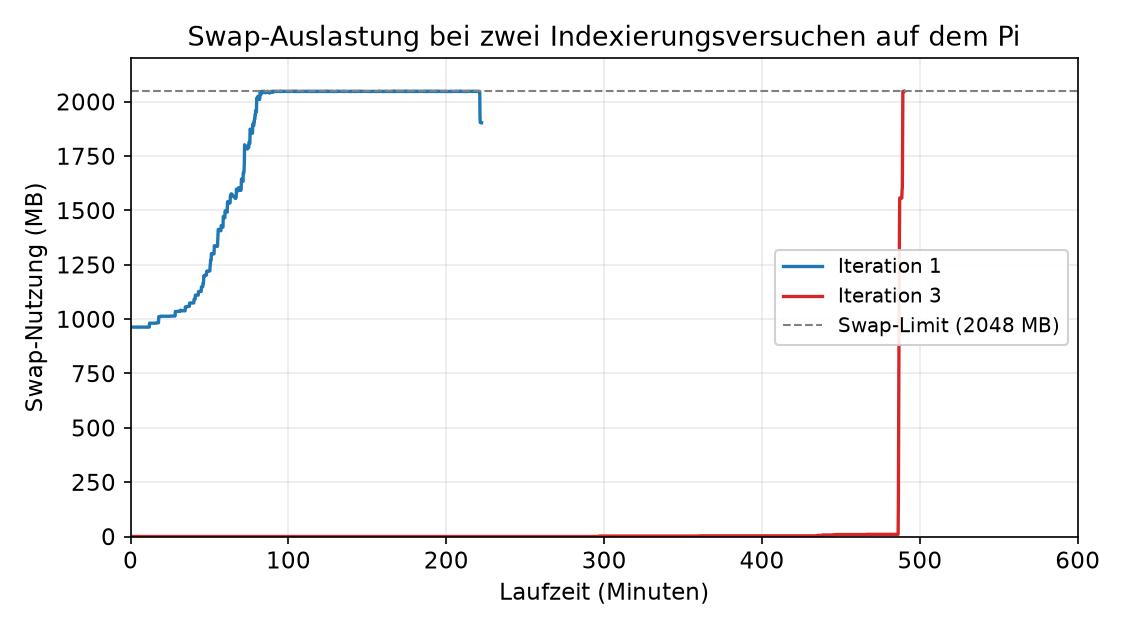
\includegraphics[width=0.9\textwidth]{swap_vergleich.pdf}
    \caption{Swap-Auslastung bei zwei der drei Indexierungsversuche auf dem Raspberry Pi: Iteration~1 mit allmählichem Anstieg über rund 85 Minuten, Iteration~3 mit langer stabiler Phase (ca. 8 Stunden) und anschließendem abrupten Kollaps.}
    \label{fig:swap-vergleich}
\end{figure}

\section{Entscheidung: Trennung von Build- und Serve-Phase}
\label{sec:build-serve-split}

Die Aufgabenstellung verlangt, dass die fertige Lösung auf dem Pi läuft, nicht zwingend, dass der Pi den Indexierungsprozess selbst durchführt. Diese Unterscheidung ist der eigentliche Grund, 
warum die in Abschnitt~\ref{sec:speicherbedarf} beschriebenen Speicherprobleme am Ende kein Blocker blieben: Sie mussten nicht auf dem Pi gelöst werden, sondern nur so weit, dass 
irgendeine verfügbare Hardware den vollen Korpus verarbeiten kann.

Der volle englischsprachige Wikipedia-Dump wird deshalb nicht auf dem Pi, sondern auf einem eigens dafür angefragten, deutlich leistungsfähigeren Server indexiert 
(104 CPU-Kerne, rund 755~GB RAM). Der fertige OpenSearch-Index wird anschließend per Snapshot vom Server auf den Pi übertragen, über denselben \texttt{path.repo}-Mechanismus, der 
bereits in Abschnitt~\ref{sec:opensearch-index-design} beschrieben wurde. Auf dem Pi selbst muss folglich nur noch der bereits fertige Index eingespielt und für Anfragen bereitgestellt 
werden; die rechenintensive Aufbauphase entfällt dort vollständig.

Angefragt wurde der Server erst, nachdem die in Abschnitt~\ref{sec:speicherbedarf} beschriebenen Läufe auf dem Pi wiederholt im vollen Swap endeten. 
Mit welcher genauen OpenSearch-Konfiguration (Heap-Größe, Ressourcen-Limits) der Index letztlich auf dem Pi betrieben wird, lässt sich aus dem aktuellen 
Repository-Stand nicht ablesen: Das lokale \texttt{docker-compose.yml} deckt nachweislich nur den Entwicklungsaufbau ab, nicht den tatsächlichen Pi-Betrieb. Bekannt ist 
lediglich, dass die Indexierung selbst auf dem Server erfolgte, nicht mit welchen exakten Parametern der Pi den übertragenen Index anschließend bedient.

\section{Monitoring-Infrastruktur}

Für die in Abschnitt~\ref{sec:speicherbedarf} beschriebenen Läufe wurde der Ressourcenverbrauch über \texttt{monitor\_run.py} aufgezeichnet. 
Das Skript tastet in einem konfigurierbaren Intervall (Standard: 10 Sekunden) Systemmetriken ab und schreibt sie als CSV-Zeile fort, während 
der eigentliche Indexierungslauf in einem separaten Prozess läuft.

Bewusst stdlib-only: Das Skript liest direkt aus \texttt{/proc/meminfo} und \texttt{/proc/vmstat} statt eine Bibliothek wie \texttt{psutil} 
einzubinden, und lässt sich unabhängig vom \texttt{wikipod}-Package installieren beziehungsweise ausführen. Dadurch ist kein zusätzlicher 
Installationsschritt auf dem Pi nötig, und es entsteht kein Konfliktrisiko mit der virtuellen Umgebung, die für den eigentlichen Indexierungslauf 
genutzt wird.

Erfasst werden pro Zeitpunkt: Load Average über 1 und 5 Minuten, eine daraus abgeleitete CPU-Auslastung (Load im Verhältnis zur Kernzahl), 
Gesamt- und verfügbarer Arbeitsspeicher, die aufsummierte RSS aller Prozesse, deren Kommandozeile \texttt{wikipod} beziehungsweise 
\texttt{opensearch} enthält, sowie belegter und verfügbarer Swap-Speicher inklusive Swap-In/Out-Seiten. Auf dem Pi kommen CPU-Temperatur 
und Throttling-Status über \texttt{vcgencmd} hinzu; auf anderen Systemen liefert derselbe Aufruf kontrolliert \texttt{None} zurück, statt 
das Skript abzubrechen.

Ein praktisches Detail betrifft die Ausgabe: Ein erneuter Aufruf mit demselben \texttt{--out}-Pfad hängt an die bestehende CSV an, 
statt sie zu überschreiben. Ein Neustart des Monitors nach einem Absturz verliert dadurch keine bereits aufgezeichneten Samples — genau das erklärt 
auch, warum sich in einigen der aufgezeichneten Läufe (Abschnitt~\ref{sec:speicherbedarf}) bereits zu Beginn ein teilweise gefüllter Swap-Speicher 
zeigt, wenn zwischen zwei Versuchen kein Neustart des Systems selbst erfolgte.

Als Auswertungsgegenstück liest \texttt{plot\_metrics.py} eine solche CSV ein und erzeugt daraus sowohl Kennzahlen (Spitzenwerte, Laufzeit) als 
auch die in diesem Kapitel verwendeten Diagramme.
\chapter{Evaluation}
\label{ch:evaluation}

\section{Effektivität: Retrieval-Qualität}

Zur Bewertung der Retrieval-Qualität wurden zwei manuell
zusammengestellte Evaluationsdatensätze verwendet. Der reguläre
Evaluationsdatensatz umfasst 20 natürlichsprachliche Suchanfragen aus
verschiedenen Themenbereichen, darunter Geschichte, Politik und Gesellschaft,
Biologie und Medizin, Naturwissenschaften, Geografie, Technologie und Kultur.
Für jede Anfrage wurde ein erwarteter Wikipedia-Artikel als Ground Truth
hinterlegt.

Ergänzend wurde ein separater Edge-Case-Datensatz erstellt. Dieser enthält
gezielt Anfragen, bei denen besondere Schwierigkeiten für das Retrieval zu
erwarten sind. Dazu gehören ähnlich benannte Entitäten, Aliase beziehungsweise
alternative Bezeichnungen, Tippfehler, sehr kurze Suchanfragen sowie eine
Anfrage zu einem Thema außerhalb des verwendeten Korpus. Die Edge Cases wurden getrennt
vom regulären Evaluationsdatensatz betrachtet, da sie nicht die allgemeine
Retrieval-Qualität abbilden, sondern gezielt das Verhalten des Systems in
problematischen Situationen untersuchen.

Als Retrieval-Ergebnis werden die ersten $k$ unterschiedlichen
Wikipedia-Artikel betrachtet. Da ein Artikel im Vektorindex durch mehrere
Text-Chunks repräsentiert werden kann, werden mehrere Treffer desselben
Artikels bei der Evaluation zu einem Artikeltreffer zusammengefasst.

Zur quantitativen Bewertung werden Recall@k, Precision@k, nDCG@k und der
Mean Reciprocal Rank (MRR) verwendet. Recall@k beschreibt den Anteil der
relevanten Artikel, die innerhalb der ersten $k$ Ergebnisse gefunden werden.
Precision@k misst den Anteil relevanter Treffer unter den ersten $k$
Ergebnissen. nDCG@k berücksichtigt zusätzlich die Position eines relevanten
Treffers und bewertet früher platzierte Treffer höher. Der Reciprocal Rank
entspricht dem Kehrwert des Rangs des ersten relevanten Treffers; der MRR
bildet den Mittelwert dieses Wertes über alle Evaluationsanfragen.

Formal sei $G$ die Menge der relevanten Ground-Truth-Artikel und
$R_k$ die Menge der ersten $k$ Retrieval-Ergebnisse. Dann ist Recall@k
definiert als

\[
\mathrm{Recall@k} = \frac{|R_k \cap G|}{|G|},
\]

während Precision@k durch

\[
\mathrm{Precision@k} = \frac{|R_k \cap G|}{k}
\]

\par\smallskip
\noindent\begin{minipage}[t]{\linewidth}
gegeben ist. Für nDCG@k wird die Position relevanter Treffer
berücksichtigt. Bei binärer Relevanz wird zunächst

\[
\mathrm{DCG@k} =
\sum_{i=1}^{k}
\frac{\mathrm{rel}_i}{\log_2(i+1)}
\]
\end{minipage}\par\smallskip

berechnet und anschließend durch den idealen DCG-Wert normalisiert:

\[
\mathrm{nDCG@k} =
\frac{\mathrm{DCG@k}}{\mathrm{IDCG@k}}.
\]

Der Reciprocal Rank einer Anfrage ist

\[
\mathrm{RR} = \frac{1}{r},
\]

wobei $r$ dem Rang des ersten relevanten Treffers entspricht. Wird kein
relevanter Artikel gefunden, ist der Wert 0. Der Mean Reciprocal Rank ergibt
sich als Mittelwert der Reciprocal-Rank-Werte über alle Anfragen.

Die Metriken betrachten unterschiedliche Aspekte der Retrieval-Qualität.
Recall@k zeigt, ob die relevanten Artikel innerhalb der betrachteten
Ergebnisse gefunden werden, während Precision@k den Anteil relevanter
Treffer innerhalb dieser Ergebnisse beschreibt. nDCG@k und MRR
berücksichtigen zusätzlich die Rangposition und unterscheiden damit
zwischen relevanten Treffern, die früh oder erst später in der
Ergebnisliste erscheinen.

\section{Effektivität: Ergebnisse}

Für den regulären Evaluationsdatensatz wurde das Retrieval zunächst mit
$k=5$ und anschließend mit $k=10$ ausgewertet. Bei beiden Einstellungen
wurden für alle 20 Anfragen die jeweils als relevant definierten
Wikipedia-Artikel innerhalb der betrachteten Treffer gefunden. Damit wurde
sowohl für $k=5$ als auch für $k=10$ ein mittlerer Recall von $1{,}000$
erreicht. Der MRR betrug in beiden Fällen $0{,}950$, der mittlere nDCG-Wert
$0{,}963$.

\begin{table}[ht]
    \centering
    \caption{Retrieval-Ergebnisse des regulären Evaluationsdatensatzes}
    \label{tab:retrieval-regulaer}
    \begin{tabular}{lrrrr}
        \toprule
        Einstellung & Recall@k & Precision@k & nDCG@k & MRR \\
        \midrule
        $k=5$  & 1,000 & 0,200 & 0,963 & 0,950 \\
        $k=10$ & 1,000 & 0,100 & 0,963 & 0,950 \\
        \bottomrule
    \end{tabular}
\end{table}

Die mittlere Precision betrug bei $k=5$ $0{,}200$ und bei $k=10$
$0{,}100$. Dieser Rückgang ist durch die Struktur des Evaluationsdatensatzes
zu erklären: Für jede der 20 Anfragen ist genau ein relevanter
Ground-Truth-Artikel definiert. Wird dieser gefunden, beträgt die
Precision daher bei fünf betrachteten Ergebnissen $1/5$ und bei zehn
betrachteten Ergebnissen $1/10$. Die Erhöhung von $k$ von 5 auf 10 führte
somit auf diesem Datensatz zu keiner Verbesserung von Recall, nDCG oder MRR.

Zusätzlich wurde das Retrieval auf dem separaten Edge-Case-Datensatz mit
zwölf Anfragen bei $k=5$ untersucht. Ohne Query Analyzer wurden ein
mittlerer Recall@5 von $0{,}833$, eine Precision@5 von $0{,}167$, ein
nDCG@5 von $0{,}803$ und ein MRR von $0{,}792$ erreicht. Mit aktiviertem Query Analyzer stiegen diese Werte auf $0{,}917$, $0{,}183$,
$0{,}886$ beziehungsweise $0{,}875$. Gegenüber der Baseline entspricht dies
einer absoluten Verbesserung von $0{,}083$ bei Recall@5, nDCG@5 und MRR sowie
von $0{,}017$ bei Precision@5.

\begin{table}[ht]
    \centering
    \caption{Retrieval-Ergebnisse auf dem Edge-Case-Datensatz bei $k=5$}
    \label{tab:retrieval-edge-cases}
    \begin{tabular}{lrrrr}
        \toprule
        Einstellung & Recall@5 & Precision@5 & nDCG@5 & MRR \\
        \midrule
        Ohne Query Analyzer & 0,833 & 0,167 & 0,803 & 0,792 \\
        Mit Query Analyzer  & 0,917 & 0,183 & 0,886 & 0,875 \\
        \bottomrule
    \end{tabular}
\end{table}

Die Verbesserung ist in diesem Versuch auf die Anfrage
\texttt{Cathlic Chuch} zurückzuführen. Ohne Vorverarbeitung wurde der
erwartete Artikel innerhalb der ersten fünf Ergebnisse nicht gefunden.
Der Query Analyzer normalisierte diese Anfrage zu
\texttt{Catholic Church}; anschließend wurde der erwartete Artikel auf
Rang 1 gefunden. Andere untersuchte Edge Cases, beispielsweise
\texttt{Who was George IV?}, wurden durch diese Normalisierung nicht
verändert.

Der Edge-Case-Datensatz enthält außerdem eine als Out-of-Scope markierte
Anfrage zu Albert Einstein, für die kein relevanter Ground-Truth-Artikel
definiert ist. Die aktuelle Implementierung der klassischen
Retrieval-Metriken weist einer Anfrage ohne relevante Ground-Truth-Titel
den Wert 0 zu. Dieser Fall ist daher nicht als gewöhnlicher
Retrieval-Fehler zu interpretieren und muss bei der Einordnung der
aggregierten Edge-Case-Werte gesondert berücksichtigt werden.

\section{Effizienz: Indexierung}

Die Ressourcennutzung während eines Indexierungslaufs auf dem Raspberry Pi
wurde in Intervallen von zehn Sekunden aufgezeichnet. Erfasst wurden unter
anderem die systemweite Speichernutzung, der RSS-Speicherbedarf des
WikiPod-Prozesses und von OpenSearch, die Swap-Nutzung sowie CPU-Temperatur
und Systemlast.

Während der aufgezeichneten Messung lag die maximale systemweite
Speichernutzung bei $6224{,}3$ MB. Für den WikiPod-Prozess wurde ein
maximaler RSS-Wert von $2871{,}1$ MB und für OpenSearch ein maximaler
RSS-Wert von $4731{,}6$ MB gemessen. Die beiden RSS-Maximalwerte traten
nicht notwendigerweise zum selben Zeitpunkt auf und werden daher nicht
addiert. Während der gesamten Messung wurde kein Swap-Speicher verwendet.
Die höchste gemessene CPU-Temperatur betrug $71{,}4\,^\circ$C.

Die Monitoring-Aufzeichnung umfasst insgesamt 62 Messpunkte über einen
Zeitraum von etwa $10{,}2$ Minuten. Dieser Zeitraum ist nicht mit der
exakten Indexierungsdauer gleichzusetzen, da das Monitoring vor dem
eigentlichen Lauf gestartet und nach dessen Ende beendet wurde.

Ergänzend wurde die Indexierungsdauer auf dem Raspberry Pi in einem
separaten Lauf direkt als Wall-Clock-Zeit gemessen. Hierfür wurde derselbe
Top-100-ZIM-Korpus mit 194 Artikeln verwendet. Bei einem konfigurierten
Speicherbudget von $500$ MB wurden $61{,}6$ MB Inhalt ausgewählt und
insgesamt 3875 Text-Chunks erzeugt und in einen separaten OpenSearch-Index
geschrieben. Die gesamte Indexierung dauerte $606{,}76$ Sekunden, entsprechend
etwa $10$ Minuten und $7$ Sekunden.

Ergänzend wurde die Indexierung des für die Retrieval-Evaluation verwendeten
Top-100-ZIM-Korpus lokal reproduziert. Aus dem Korpus wurden 194 von 194
verfügbaren Artikeln ausgewählt. Der dabei berücksichtigte Inhalt umfasste
$61{,}6$ MB bei einem konfigurierten Speicherbudget von $500$ MB. Aus den
Artikeln wurden insgesamt 3875 Text-Chunks erzeugt und in OpenSearch
indexiert. Der resultierende OpenSearch-Index enthielt entsprechend 3875
Dokumente und belegte $42{,}1$ MB Speicherplatz.

Dieser lokale Lauf dient der Reproduzierbarkeit der für die
Retrieval-Evaluation verwendeten Indexbasis. Die zuvor beschriebenen
Ressourcenmessungen stammen dagegen vom Raspberry Pi und werden daher nicht
direkt mit den lokal gemessenen Werten vermischt.


\section{Effizienz: Anfragebearbeitung}

Die Latenz der Retrieval-Stufe wurde zusätzlich in einem lokalen
Reproduktionslauf mit den 20 Anfragen des regulären Evaluationsdatensatzes
und $k=5$ gemessen. Dabei wurde jeweils der vollständige Aufruf der
Retrieval-Komponente erfasst, der sowohl die Berechnung des Query-Embeddings
als auch die anschließende $k$-NN-Suche in OpenSearch umfasst. Ein
vorangestellter Warm-up-Aufruf wurde nicht in die Messwerte einbezogen.

Die mittlere Retrieval-Latenz betrug $27{,}13$ ms pro Anfrage, bei einem
Median von $28{,}73$ ms. Die gemessenen Einzelwerte lagen zwischen
$15{,}99$ ms und $41{,}26$ ms. Da diese Messung auf dem lokalen
Entwicklungssystem und nicht auf dem Raspberry Pi durchgeführt wurde,
dienen die Werte der Charakterisierung des Evaluationsaufbaus und sind
nicht als Laufzeitmessung der Zielhardware zu interpretieren.

Die gleiche Retrieval-Messung wurde anschließend auf dem Raspberry Pi
wiederholt. Verwendet wurden ebenfalls die 20 Anfragen des regulären
Evaluationsdatensatzes, $k=5$ und ein vorangestellter Warm-up-Aufruf, der
nicht in die Messwerte einbezogen wurde. Gemessen wurde wiederum der
vollständige Aufruf der Retrieval-Komponente einschließlich
Query-Embedding und $k$-NN-Suche in OpenSearch.

Auf dem Raspberry Pi betrug die mittlere Retrieval-Latenz $62{,}78$ ms
pro Anfrage bei einem Median von $53{,}76$ ms. Die Einzelwerte lagen
zwischen $46{,}40$ ms und $115{,}56$ ms. Damit lag die mittlere
Retrieval-Latenz in diesem Versuchsaufbau auf dem Raspberry Pi etwa beim
$2{,}31$-Fachen des lokal gemessenen Mittelwerts von $27{,}13$ ms.

Zur Untersuchung der Generierungslatenz wurden auf dem Raspberry Pi drei
lokale Sprachmodelle im GGUF-Format verglichen. Für jedes Modell wurden
dieselben 20 Anfragen des regulären Evaluationsdatensatzes verwendet.
Das Retrieval wurde dabei einmal pro Anfrage ausgeführt und für alle
Modelle wiederverwendet. Die gemessene Zeit umfasst daher ausschließlich
den Aufruf der Generierung und nicht die Retrieval-Latenz.

\begin{table}[ht]
    \centering
    \caption{Mittlere Generierungslatenz lokaler Sprachmodelle auf dem Raspberry Pi}
    \label{tab:pi-generation-latency}
    \begin{tabular}{lrr}
        \toprule
        Modell & Modellgröße & Mittlere Latenz \\
        \midrule
        Llama 3.2 1B Q4 & 771 MB & 29,18 s \\
        Phi-3.5 Mini Q4 & 2,3 GB & 152,33 s \\
        Qwen2.5 1.5B Q4 & 1,1 GB & 27,97 s \\
        \bottomrule
    \end{tabular}
\end{table}

In diesem Versuchsaufbau erreichte Qwen2.5 1.5B mit $27{,}97$ Sekunden
die niedrigste mittlere Generierungslatenz, knapp vor Llama 3.2 1B mit
$29{,}18$ Sekunden. Phi-3.5 Mini benötigte mit $152{,}33$ Sekunden
deutlich mehr Zeit. Die Messung bewertet ausschließlich die Laufzeit der
Generierung; aus diesen Werten kann keine Aussage über die Qualität der
generierten Antworten abgeleitet werden.

Ergänzend wurde die Ressourcennutzung während einer einzelnen
Generierung mit Qwen2.5 1.5B auf dem Raspberry Pi in Intervallen von zwei
Sekunden aufgezeichnet. Die Generierung dauerte in diesem Lauf
$27{,}42$ Sekunden. Die systemweite Speichernutzung stieg von
$4577{,}8$ MB vor der Generierung auf maximal $5770{,}7$ MB und lag am
Ende der Messung bei $4593{,}5$ MB. Gegenüber dem Ausgangswert entspricht
dies einem Anstieg bis zum Maximum von etwa $1192{,}9$ MB.

Die Swap-Belegung lag bereits vor Beginn der Generierung bei etwa
$2048$ MB. Während des Messzeitraums wurden zwei zusätzliche
Swap-In-Seiten und keine Swap-Out-Seiten registriert. Die bereits
vorhandene Swap-Belegung kann daher nicht der untersuchten Generierung
zugeschrieben werden. Die CPU-Temperatur stieg während der Messung von
$44{,}4\,^\circ$C auf maximal $56{,}0\,^\circ$C und lag am Ende bei
$46{,}1\,^\circ$C.

Der separat erfasste RSS-Wert des WikiPod-Prozesses bildet in diesem Lauf
den Speicherbedarf der eigentlichen Modellgenerierung nicht verlässlich
ab. Aus diesem Grund wird für diese Messung nur die Veränderung der
systemweiten Speichernutzung berichtet und nicht daraus auf den
prozessspezifischen Speicherbedarf des Sprachmodells geschlossen.

\section{Einordnung der Ergebnisse}

Die Ergebnisse zeigen für den regulären Evaluationsdatensatz eine hohe
Retrieval-Qualität. Die Aussagekraft ist jedoch durch den Umfang des
Evaluationsaufbaus begrenzt. Der reguläre Datensatz umfasst lediglich
20 Anfragen und definiert für jede Anfrage genau einen relevanten
Ground-Truth-Artikel. Die gemessenen Werte sind daher als Ergebnis dieses
konkreten Evaluationsdatensatzes zu verstehen und erlauben keine allgemeine
Aussage über beliebige Wikipedia-Anfragen.

Auch der verwendete Korpus ist begrenzt. Für die reproduzierte
Retrieval-Evaluation wurde eine Top-100-ZIM-Datei mit einer Dateigröße von
318 MB verwendet. Beim Einlesen wurden daraus 194 Artikel verarbeitet und
3875 Chunks erzeugt. Die Ergebnisse können deshalb nicht unmittelbar auf
einen wesentlich größeren Wikipedia-Korpus übertragen werden.

Der Edge-Case-Datensatz verdeutlicht zudem, dass die aggregierten Metriken
von der Definition der Ground Truth abhängen. Insbesondere erhält die
Out-of-Scope-Anfrage ohne relevante Ground-Truth-Titel in der aktuellen
Implementierung für die klassischen Retrieval-Metriken jeweils den Wert
0. Sie muss deshalb getrennt von gewöhnlichen Retrieval-Fehlern
interpretiert werden.

\begingroup
\emergencystretch=1em
Der zusätzlich eingesetzte LLM-Judge erwies sich in der aktuellen
Konfiguration nur eingeschränkt als quantitative Bewertungsmetrik. In einem
frischen Lauf auf dem Edge-Case-Datensatz wurden insgesamt 22
Retrieval-Ergebnisse bewertet. Dabei vergab der Judge viermal den Wert 0, zweimal den
Wert 1, fünfzehnmal den Wert 2 und einmal den Wert 3 auf einer Skala von 0
bis 3.\par
\endgroup

Die Einzelbewertungen zeigen jedoch mehrere Inkonsistenzen. So wurde bei der
Anfrage \texttt{Who was George IV?} auch ein Treffer zum Artikel
\texttt{George III} mit 2 von 3 Punkten bewertet. Bei der Anfrage \texttt{Cathlic Chuch} wurde der nach der
Retrieval-Normalisierung korrekt gefundene Artikel \texttt{Catholic Church}
dagegen mit 0 Punkten bewertet. Der Judge erhielt dabei die ursprüngliche
Anfrage und nicht die für das Retrieval normalisierte Form. Auch bei der als
Out-of-Scope definierten Anfrage zu Albert Einstein erhielt ein Treffer zum
Artikel \texttt{Martin Luther King Jr.} 2 Punkte. Die Judge-Bewertungen werden
daher nicht als gleichwertige quantitative Qualitätsmetrik neben Recall,
nDCG und MRR verwendet, sondern als experimentelle Ergänzung betrachtet.

Die Messungen auf dem Raspberry Pi zeigen zudem deutliche Unterschiede
zwischen Retrieval und Antwortgenerierung hinsichtlich der Laufzeit. Die
mittlere Retrieval-Latenz lag mit $62{,}78$ ms deutlich unter einer Sekunde,
während die untersuchten lokalen Sprachmodelle für die Generierung einer
Antwort im Mittel zwischen $27{,}97$ s und $152{,}33$ s benötigten. In dem
untersuchten Aufbau stellt damit die lokale Sprachmodellgenerierung den
zeitlich dominierenden Teil der Anfragebearbeitung dar.

Auch zwischen den untersuchten Sprachmodellen bestanden deutliche
Laufzeitunterschiede. Qwen2.5 1.5B erreichte mit $27{,}97$ s die niedrigste
mittlere Generierungslatenz, gefolgt von Llama 3.2 1B mit $29{,}18$ s.
Phi-3.5 Mini benötigte dagegen im Mittel $152{,}33$ s. Da in diesem
Modellvergleich keine quantitative Qualitätsmetrik für die generierten
Antworten erhoben wurde, lässt sich aus der geringeren Latenz allein keine
Aussage über die Eignung eines Modells hinsichtlich der Antwortqualität
ableiten.

Die Ressourcenmessung einer einzelnen Qwen2.5-Generierung zeigte einen
Anstieg der systemweiten Speichernutzung um maximal etwa $1{,}19$ GB
gegenüber dem Ausgangswert. Dabei wurde keine relevante zusätzliche
Swap-Out-Aktivität beobachtet. Da der prozessspezifische Speicherbedarf
der Modellgenerierung in dieser Messung nicht verlässlich erfasst wurde,
ist dieser Wert als Veränderung der gesamten Systemspeichernutzung und
nicht als direkter Speicherbedarf des Modells zu interpretieren.
\chapter{Anleitung: Inbetriebnahme}
\label{ch:anleitung}

Dieses Kapitel beschreibt die grundlegenden Schritte zur Inbetriebnahme von
WikiPod. Die Anleitung ist insbesondere als Einstiegspunkt für Folgeprojekte
gedacht. Weiterführende Informationen zur Projektstruktur und zu einzelnen
Komponenten befinden sich in der README-Datei des Repositorys.

\section{Voraussetzungen}

Für die lokale Ausführung wird eine Python-Umgebung sowie Docker mit Docker
Compose benötigt. Die Anwendung verwendet OpenSearch für die Speicherung und
Abfrage der erzeugten Vektorrepräsentationen. Für die Dokumentengrundlage wird
außerdem eine lokale Wikipedia-ZIM-Datei benötigt. Diese ist aufgrund ihrer
Größe nicht Bestandteil des Repositorys und muss separat bereitgestellt werden.

Für den produktionsnahen Betrieb wurde im Projekt ein Raspberry Pi~5 mit
16\,GB Arbeitsspeicher und einer 1-TB-SSD verwendet. Die grundlegenden
Entwicklungs- und Testschritte können jedoch auch auf einem gewöhnlichen
Entwicklungsrechner durchgeführt werden.

\section{Installation}

Nach dem Klonen des Repositorys wird zunächst eine virtuelle Python-Umgebung
erstellt und anschließend das Projekt einschließlich der
Entwicklungsabhängigkeiten installiert.

\begin{lstlisting}[language=bash]
git clone https://github.com/niklasbelieres/wikipod-rag
cd wikipod-rag

python -m venv .venv
source .venv/bin/activate
pip install -e ".[dev]"
\end{lstlisting}

Anschließend muss eine Wikipedia-ZIM-Datei lokal bereitgestellt werden. Der
Pfad zu dieser Datei wird über den Eintrag \texttt{paths.zim\_file} in der
jeweiligen Konfigurationsdatei festgelegt.

\section{Lokales Setup (Entwicklung)}

OpenSearch wird lokal über Docker Compose gestartet:

\begin{lstlisting}[language=bash]
docker compose up -d
\end{lstlisting}

Ob OpenSearch erreichbar ist, kann anschließend beispielsweise mit folgendem
Aufruf geprüft werden:

\begin{lstlisting}[language=bash]
curl http://localhost:9200
\end{lstlisting}

Wenn die konfigurierte ZIM-Datei vorhanden und OpenSearch gestartet ist, kann
die Indexierung im Entwicklungsmodus ausgeführt werden:

\begin{lstlisting}[language=bash]
WIKIPOD_ENV=dev python -m wikipod.cli index
\end{lstlisting}

Nach erfolgreicher Indexierung kann eine Anfrage an das System gestellt werden:

\begin{lstlisting}[language=bash]
WIKIPOD_ENV=dev python -m wikipod.cli query \
  "What is the Catholic Church?"
\end{lstlisting}

Soll ausschließlich das Retrieval untersucht werden, ohne eine Antwort durch
das lokale Sprachmodell zu erzeugen, kann die Option
\texttt{--chunks-only} verwendet werden:

\begin{lstlisting}[language=bash]
WIKIPOD_ENV=dev python -m wikipod.cli query \
  --chunks-only "What is the Catholic Church?"
\end{lstlisting}

\section{Konfiguration}

Die Konfiguration des Systems befindet sich im Verzeichnis
\texttt{config/}. Unterschiedliche Konfigurationen werden für Entwicklung,
Evaluation, Tests auf dem Raspberry Pi und den produktionsnahen Betrieb
verwendet. Über die Umgebungsvariable \texttt{WIKIPOD\_ENV} kann die jeweils
benötigte Laufzeitkonfiguration ausgewählt werden. Wird keine Umgebung
angegeben, verwendet WikiPod standardmäßig die Entwicklungsumgebung
\texttt{dev}.

Insbesondere muss der Pfad zur verwendeten Wikipedia-ZIM-Datei über
\texttt{paths.zim\_file} an die lokale Umgebung angepasst werden. Dadurch
können unterschiedliche Datensätze und Laufzeitumgebungen verwendet werden,
ohne die allgemeine Projektkonfiguration für jeden Versuch verändern zu
müssen.

\section{Deployment auf dem Raspberry Pi}

Für den Betrieb auf dem Raspberry Pi wird das Repository zunächst auf das
Gerät übertragen und analog zur lokalen Installation eingerichtet. Die
Wikipedia-ZIM-Datei muss auf dem lokalen Speichermedium des Raspberry Pi
vorliegen und der entsprechende Pfad in der dafür vorgesehenen
Konfiguration eingetragen werden.

OpenSearch wird auch auf dem Raspberry Pi über Docker Compose betrieben.
Nach dem Start von OpenSearch kann die Indexierung mit der für den jeweiligen
Versuch vorgesehenen Konfiguration ausgeführt werden. Für Pi-spezifische
Testläufe steht beispielsweise die Konfiguration
\texttt{config/pi-test.yaml} zur Verfügung. Dadurch können Experimente auf dem
Raspberry Pi durchgeführt werden, ohne die Standardkonfiguration für die
Entwicklung zu verändern.

\par\smallskip
\noindent\begin{minipage}[t]{\linewidth}
Bei längeren Indexierungsläufen kann zusätzlich das im Projekt enthaltene
Monitoring gestartet werden:

\begin{lstlisting}[language=bash]
python -m wikipod.scripts.monitor_run \
  --out logs/pi_top100_index.csv \
  --interval 10
\end{lstlisting}
\end{minipage}\par\smallskip

Das Monitoring zeichnet unter anderem CPU-, Speicher-, Swap- und
Temperaturwerte sowie den Speicherverbrauch von WikiPod und OpenSearch auf.
Nach Abschluss des Laufs kann das Monitoring mit \texttt{Ctrl+C} beendet und
die erzeugte CSV-Datei ausgewertet werden:

\begin{lstlisting}[language=bash]
python -m wikipod.scripts.plot_metrics \
  logs/pi_top100_index.csv
\end{lstlisting}

\section{Evaluation ausführen}

Für die Retrieval-Evaluation steht das Kommando \texttt{evaluate} zur
Verfügung. Als Eingabe wird ein YAML- oder JSON-Datensatz mit
natürlichsprachlichen Anfragen und den jeweils relevanten Wikipedia-Artikeln
verwendet.

Für die im Bericht eingesetzte Evaluationskonfiguration kann beispielsweise
folgender Aufruf ausgeführt werden:

\begin{lstlisting}[language=bash]
WIKIPOD_ENV=report_eval python -m wikipod.cli evaluate \
  --dataset test/data/eval_queries.yaml
\end{lstlisting}

Die Anzahl der betrachteten Retrieval-Ergebnisse kann bei Bedarf mit
\texttt{--top-k} überschrieben werden. Ergebnisse lassen sich außerdem als
JSON oder CSV beziehungsweise gesammelt in einem Ausgabeverzeichnis speichern:

\begin{lstlisting}[language=bash]
WIKIPOD_ENV=report_eval python -m wikipod.cli evaluate \
  --dataset test/data/eval_queries.yaml \
  --top-k 5 \
  --output-dir logs/report_eval_k5
\end{lstlisting}

Optional können mit \texttt{--use-query-analyzer} die normalisierten Anfragen
des Query Analyzers verwendet und mit \texttt{--use-llm-judge} zusätzliche
LLM-basierte Bewertungen aktiviert werden.

Vor einem neuen Lauf können die automatisierten Tests und die statische
Codeprüfung ausgeführt werden:

\begin{lstlisting}[language=bash]
pytest
ruff check .
\end{lstlisting}

Diese Prüfungen werden zusätzlich bei Pushes und Pull Requests auf den
\texttt{main}-Branch über GitHub Actions ausgeführt.
\chapter{Diskussion}
\label{ch:diskussion}
% Reflektierender Teil -- oft unterschaetzt, aber genau das, was einen
% guten von einem rein beschreibenden Bericht unterscheidet.

\section{Herausforderungen}
% Die Speicher-Eskalation (Kap. 6) als zentrales Beispiel: naheliegende
% Erstdiagnosen trafen jeweils einen echten, aber nicht dominanten Faktor --
% erst die Frage "wie viele Objekte leben gleichzeitig" fuehrte zur Loesung.
% Das ist eine uebertragbare Erkenntnis, nicht nur eine Randnotiz.
Eine zentrale Herausforderung bei der Verarbeitung des vollständigen
Wikipedia-Korpus war der stark ansteigende Speicherbedarf. Während die
Verarbeitung kleinerer Datenmengen zunächst unauffällig verlief, zeigte sich
beim Skalieren auf den vollständigen Korpus, dass zuvor verwendete
In-Memory-Ansätze nicht ausreichend skalieren. Die Fehlersuche konzentrierte
sich zunächst auf einzelne speicherintensive Datenstrukturen und
Verarbeitungsschritte. Diese Faktoren trugen zwar zum Speicherverbrauch bei,
erklärten dessen Größenordnung jedoch nicht vollständig.

Entscheidend war letztlich nicht allein die Größe einzelner Objekte, sondern
die Anzahl der Objekte, die während der Verarbeitung gleichzeitig im Speicher
gehalten wurden. Dadurch konnte sich ein für einen einzelnen Artikel
unkritischer Speicherbedarf über mehrere Millionen Artikel zu einem erheblichen
Gesamtspeicherbedarf aufsummieren. Diese Beobachtung führte zu einer
grundlegenderen Betrachtung der Verarbeitungspipeline: Statt lediglich einzelne
Datenstrukturen zu optimieren, musste die Lebensdauer der Daten im Speicher
reduziert werden.

Daraus ergibt sich als übertragbare Erkenntnis, dass bei der Verarbeitung
großer Korpora nicht nur die Größe einzelner Datenstrukturen betrachtet werden
sollte. Ebenso relevant ist, wie viele dieser Strukturen gleichzeitig
existieren und zu welchem Zeitpunkt sie wieder freigegeben werden können. Für
WikiPod war diese Erkenntnis insbesondere für die Skalierung vom kleinen
Evaluationskorpus auf den vollständigen Wikipedia-Bestand von Bedeutung und
motivierte eine stärker streamingorientierte Verarbeitung, bei der
Zwischenergebnisse möglichst früh weiterverarbeitet beziehungsweise
persistiert werden, anstatt sie über den gesamten Verarbeitungslauf im
Arbeitsspeicher zu halten.

\section{Designentscheidungen im Rueckblick}
% Was wuerdet ihr nochmal genauso machen, was anders (z. B. frueher auf
% Streaming-Architektur setzen statt erst bei vollem Korpus zu merken,
% dass In-Memory-Ansaetze nicht skalieren).

Ein konkreter Punkt, den wir im Rückblick anders angehen würden, betrifft die Gewichtung des Scoring-Modells
aus Abschnitt~\ref{ch:dokumentenauswahl}. Die Messung auf dem vollen en.wikipedia-Korpus (Tabelle~\ref{tab:scoring-weights})
zeigt, dass \texttt{importance} trotz eines mit 0,150 vergleichsweise niedrigen Gewichts 82,61\,\% des
gewichteten Gesamtscores ausmacht, während \texttt{incoming\_links} trotz des höchsten Gewichts (0,250) nur
0,31\,\% beiträgt. Ursächlich ist, dass die logarithmische Dämpfung bei \texttt{importance} pro ausgehendem
Link und nicht auf den aggregierten Artikelwert angewendet wird -- der Rohwert wächst dadurch tendenziell mit
der Anzahl der ausgehenden Links und bleibt strukturell größer als bei den übrigen, einfach gedämpften
Signalen. Die konfigurierten Gewichte spiegeln damit nicht den tatsächlichen Einfluss der Signale auf die
Auswahl wider, obwohl genau das mit \texttt{config/prod.yaml} beziehungsweise \texttt{config/server.yaml}
beabsichtigt war.

Für eine zukünftige Iteration wären zwei Ansätze naheliegend: entweder \texttt{importance} durch die Anzahl
der berücksichtigten Links zu normalisieren (Mittelwert statt Summe der gedämpften Linkfrequenzen), oder alle
fünf Rohsignale vor der Gewichtung zusätzlich zu standardisieren (z.\,B. per Z-Score relativ zu ihrer eigenen
Verteilung im Korpus), sodass ein konfiguriertes Gewicht tatsächlich einen vergleichbaren Anteil am Endscore
bewirkt -- unabhängig von der ursprünglichen Skala des jeweiligen Signals. Beide Änderungen hätten jedoch
Rückwirkungen auf die bereits durchgeführten Selektionsläufe und wurden im Rahmen dieses Projekts aus
Zeitgründen nicht mehr umgesetzt.

\section{Grenzen der Loesung}
% Was deckt das System bewusst nicht ab (z. B. nur englische Wikipedia,
% keine Multi-Turn-Konversation, Kategorien-Signal nicht genutzt, ...).

Die entwickelte Lösung unterliegt mehreren Einschränkungen, die bei der
Einordnung der Ergebnisse berücksichtigt werden müssen. Eine grundlegende
Einschränkung ergibt sich aus der verwendeten Wissensbasis. WikiPod verarbeitet
ausschließlich Inhalte der englischsprachigen Wikipedia. Andere Sprachversionen
sowie zusätzliche externe Wissensquellen werden nicht berücksichtigt. Die
verfügbaren Informationen sind damit unmittelbar durch den Inhalt und den
Stand der lokal verwendeten Wikipedia-Kopie begrenzt.

Eine weitere Einschränkung betrifft die Auswahl der lokal vorgehaltenen
Dokumente. Aufgrund des vorgegebenen Speicherbudgets kann nur ein Teil des
verfügbaren Wikipedia-Bestands berücksichtigt werden. Die Auswahl basiert auf
dem entwickelten Scoring-Verfahren und stellt daher keine Garantie dafür dar,
dass für jede mögliche Nutzeranfrage der relevanteste Artikel im lokalen
Bestand enthalten ist. Wie die Analyse des Scoring-Modells gezeigt hat,
entspricht der tatsächliche Einfluss der verwendeten Signale zudem nicht in
allen Fällen ihrer konfigurierten Gewichtung. Insbesondere die Dominanz von
\texttt{importance} kann die Zusammensetzung der ausgewählten Teilmenge
beeinflussen.

Auch die Evaluation ist in ihrer Aussagekraft begrenzt. Der reguläre
Evaluationsdatensatz umfasst 20 Anfragen und wurde ebenso wie der zusätzliche
Edge-Case-Datensatz manuell zusammengestellt. Die gemessenen Retrieval-Metriken
beschreiben daher zuverlässig das Verhalten auf den untersuchten Anfragen,
lassen sich jedoch nicht ohne Weiteres auf die Gesamtheit möglicher
Nutzeranfragen übertragen. Insbesondere seltene Themen, weitere mehrdeutige
Bezeichnungen und Anfragen außerhalb des lokal verfügbaren Wissensbestands
können in den verwendeten Datensätzen nur eingeschränkt abgebildet werden.

Darüber hinaus wurde die Qualität der generierten Antworten nicht mit einer
stabilen quantitativen Metrik bewertet. Der im Rahmen der Evaluation erprobte
LLM-Judge zeigte bei einzelnen Anfragen inkonsistente Bewertungen und wurde
deshalb nicht als alleinige Grundlage für einen quantitativen Vergleich der
Antwortqualität verwendet. Der Vergleich der lokalen Sprachmodelle erlaubt
somit vor allem Aussagen über deren Generierungslatenz auf der Zielhardware,
nicht jedoch darüber, welches Modell insgesamt die höchste inhaltliche
Antwortqualität liefert.

Schließlich setzt die lokale Ausführung auf dem Raspberry Pi der Lösung
praktische Leistungsgrenzen. Während das semantische Retrieval im untersuchten
Aufbau mit vergleichsweise geringer Latenz durchgeführt werden konnte, benötigt
die lokale Antwortgenerierung deutlich mehr Zeit und stellt damit den
dominierenden Anteil der Antwortzeit dar. Die vollständig lokale Ausführung
ermöglicht zwar den Betrieb ohne bestehende Internetverbindung, geht auf der
verwendeten Hardware jedoch mit einem deutlichen Kompromiss zwischen
Modellgröße, Ressourcenbedarf und Generierungsgeschwindigkeit einher.

\chapter{Fazit und Ausblick}
\label{ch:fazit}

\section{Fazit}
% Kurze Zusammenfassung: welche der 5 Fragestellungen wurden wie
% beantwortet, Gesamteinschaetzung.

Im Rahmen von WikiPod wurde untersucht, inwieweit sich ein lokaler Zugriff auf
ausgewählte Inhalte der englischsprachigen Wikipedia mit semantischem Retrieval
und lokaler Antwortgenerierung auf eingeschränkter Hardware umsetzen lässt.
Ausgehend von den fünf in der Aufgabenstellung formulierten Anforderungen wurde
dafür eine durchgängige Pipeline von der lokalen Wikipedia-Kopie über die
Dokumentenauswahl und Vektorindexierung bis hin zur Retrieval-Augmented-
Generation und deren Evaluation entwickelt.

Die erste Anforderung bestand in der Bereitstellung einer lokalen Kopie der
englischsprachigen Wikipedia. Hierfür werden Wikipedia-Inhalte in Form einer
lokal gespeicherten ZIM-Datei verwendet, die ohne bestehende Internetverbindung
verarbeitet werden kann. Damit bildet die ZIM-Datei die Grundlage für den
vollständig lokalen Zugriff auf den verfügbaren Wikipedia-Bestand.

Für die zweite Anforderung, die Entwicklung einer Methode zur Auswahl einer
Teilmenge der Wikipedia, wurde ein budgetbeschränktes Auswahlverfahren
implementiert. Die Artikel werden anhand mehrerer Metadaten und
Struktursignale bewertet und anschließend nach ihrem Verhältnis von Score zu
Speicherbedarf priorisiert. Im produktiven Selektionslauf auf dem vollständigen
Korpus wurden aus 7.322.195 Kandidatenartikeln 1.638.375 Artikel ausgewählt und
das konfigurierte Speicherbudget von 13.000~MB praktisch vollständig
ausgeschöpft. Die Analyse des Scoring-Modells zeigte jedoch zugleich, dass die
tatsächlichen Beiträge der einzelnen Signale nicht proportional zu ihren
konfigurierten Gewichten ausfallen. Insbesondere das Signal
\texttt{importance} besitzt einen deutlich größeren Einfluss auf den
Gesamtscore als ursprünglich durch seine Gewichtung beabsichtigt.

Die dritte Anforderung, die Indexierung der ausgewählten Teilmenge als dichte
Vektoren mittels OpenSearch, wurde durch eine Chunking- und Embedding-Pipeline
umgesetzt. Die ausgewählten Artikel werden abschnittsweise in Text-Chunks
zerlegt und mit \texttt{all-MiniLM-L6-v2} in dichte Vektorrepräsentationen
überführt \cite{minilm-model-card,sbert-pretrained-models}. Dense
Passage Retrieval zeigt grundsätzlich, dass dichte Repräsentationen für
semantisches Passage Retrieval im Open-Domain-Question-Answering eingesetzt
werden können \cite{karpukhin-etal-2020-dense}. Diese werden gemeinsam mit den
zugehörigen Metadaten in OpenSearch gespeichert. Für eingehende Nutzeranfragen
wird dasselbe Embedding-Modell verwendet, sodass über die Vektorsuche
semantisch ähnliche Textpassagen ermittelt und für die weitere Verarbeitung
bereitgestellt werden können.

Zur Beantwortung der vierten Anforderung wurden drei lokal ausführbare
Sprachmodelle auf dem Raspberry Pi hinsichtlich ihrer Generierungslatenz
verglichen. Qwen2.5~1.5B~Q4 erreichte mit durchschnittlich $27{,}97$~s die
niedrigste gemessene Generierungszeit, gefolgt von Llama~3.2~1B~Q4 mit
$29{,}18$~s und Phi-3.5~Mini~Q4 mit $152{,}33$~s. Für die Zielkonfiguration
wird daher Qwen2.5~1.5B in quantisierter Form über das
\texttt{llama\_cpp}-Backend eingesetzt. Diese Auswahl stützt sich auf die
gemessene Laufzeit und die erfolgreiche Ausführung auf der Zielhardware. Da
für den Modellvergleich keine quantitative Bewertung der Antwortqualität
durchgeführt wurde, kann daraus jedoch nicht abgeleitet werden, dass Qwen2.5
auch hinsichtlich der generierten Inhalte das qualitativ beste der
untersuchten Modelle ist.

Die fünfte Anforderung bestand in der Evaluation der entwickelten Lösung
hinsichtlich Effektivität und Effizienz. Auf dem regulären
Evaluationsdatensatz mit 20 Anfragen erreichte das Retrieval sowohl bei
$k=5$ als auch bei $k=10$ einen Recall von $1{,}000$, einen MRR von
$0{,}950$ und einen mittleren nDCG-Wert von $0{,}963$. Auf dem separaten
Edge-Case-Datensatz verbesserte der Query Analyzer den Recall@5 von
$0{,}833$ auf $0{,}917$ und den MRR von $0{,}792$ auf $0{,}875$. Die
mittlere Retrieval-Latenz auf dem Raspberry Pi betrug im untersuchten
Evaluationsaufbau $62{,}78$~ms und lag damit deutlich unter den
Generierungszeiten der lokalen Sprachmodelle. Die Antwortgenerierung stellt
somit in diesem Versuchsaufbau den zeitlich dominierenden Teil der
Anfragebearbeitung dar. Gleichzeitig ist die Aussagekraft der
Retrieval-Evaluation durch die geringe Größe und die manuelle Zusammenstellung
der verwendeten Evaluationsdatensätze begrenzt.

Zusammenfassend wurden alle fünf zentralen Anforderungen der Projektarbeit
umgesetzt beziehungsweise experimentell untersucht. Wikipedia-Inhalte können
lokal bereitgestellt, unter einem vorgegebenen Speicherbudget auf eine
Teilmenge reduziert, als dichte Vektoren in OpenSearch indexiert und für
semantisches Retrieval mit anschließender lokaler Antwortgenerierung genutzt
werden. Die Messungen zeigen, dass der grundsätzliche Betrieb der entwickelten
Pipeline auf dem Raspberry Pi möglich ist. Gleichzeitig bleiben insbesondere
die Gewichtung des Auswahlverfahrens, die begrenzte Breite der Evaluation und
die vergleichsweise hohe Laufzeit der lokalen Sprachmodellgenerierung als
wesentliche Einschränkungen der aktuellen Lösung bestehen.

\section{Ausblick}
% Was waere der naechste Schritt mit mehr Zeit -- z. B. voller Korpus auf
% dem Pi (Build/Serve-Trennung produktiv nutzen), Kategorien-basierte
% diversitaetsbewusste Selection, generierungsseitige Evaluationsmetriken
% (ROUGE/LLM-as-Judge) zusaetzlich zu Recall@k/MRR.

Ein naheliegender nächster Schritt besteht darin, die entwickelte Pipeline auf
einem deutlich größeren Wikipedia-Bestand unter der vorgesehenen
Zielkonfiguration zu betreiben. Die Architektur trennt die aufwendige
Aufbereitung und Indexierung von der späteren Nutzung des Systems, sodass ein
umfangreicher Index auf leistungsfähigerer Hardware erzeugt und anschließend
auf den Raspberry Pi übertragen werden kann. Dadurch ließe sich untersuchen,
wie sich die im kleinen Evaluationskorpus beobachteten Ergebnisse auf einen
realistischeren Datenbestand übertragen und wie sich insbesondere Indexgröße,
Speicherbedarf und Retrieval-Latenz bei wachsendem Korpus entwickeln.
Weiteres Verbesserungspotenzial besteht bei der Dokumentenauswahl. Die
Evaluation des Scoring-Verfahrens hat gezeigt, dass die tatsächlichen Beiträge
der verwendeten Signale nicht unmittelbar ihren konfigurierten Gewichten
entsprechen. Zukünftige Arbeiten sollten deshalb die Eingangssignale stärker
normalisieren und die Gewichte systematisch auf einem geeigneten
Evaluationsdatensatz bestimmen. Zusätzlich könnte eine kategorien- oder
themenbasierte Auswahl eingesetzt werden, um neben der geschätzten Relevanz
eines einzelnen Artikels auch die inhaltliche Diversität der ausgewählten
Wikipedia-Teilmenge zu berücksichtigen.
Auch die Retrieval-Evaluation sollte auf einen größeren und systematischer
zusammengestellten Datensatz erweitert werden. Neben zusätzlichen regulären
Anfragen sollten insbesondere mehrdeutige Entitäten, alternative
Bezeichnungen, Tippfehler, sehr kurze Anfragen und Out-of-Scope-Fälle stärker
vertreten sein. Für Out-of-Scope-Anfragen wäre zudem eine separate
Bewertungslogik sinnvoll, da die bisher verwendeten klassischen
Retrieval-Metriken Fälle ohne relevanten Ground-Truth-Artikel nicht angemessen
von gewöhnlichen Retrieval-Fehlern unterscheiden. Der Query Analyzer könnte
auf dieser Grundlage gezielter weiterentwickelt und seine Wirkung auf
unterschiedliche Fehlerklassen untersucht werden.
Schließlich sollte neben dem Retrieval auch die Qualität der generierten
Antworten systematisch evaluiert werden. Der bisher erprobte LLM-Judge zeigte
in einzelnen Fällen inkonsistente Bewertungen und eignet sich in seiner
aktuellen Form daher nicht als alleinige quantitative Qualitätsmetrik. Eine
zukünftige Evaluation könnte manuell bewertete Referenzantworten mit
automatisierten Verfahren kombinieren und dabei insbesondere Faktentreue,
Relevanz, Vollständigkeit und die korrekte Nutzung des bereitgestellten
Retrieval-Kontexts betrachten. Auf dieser Grundlage ließen sich die
untersuchten lokalen Sprachmodelle nicht nur hinsichtlich ihrer Laufzeit,
sondern auch hinsichtlich ihrer Antwortqualität vergleichen. Damit wäre eine
fundiertere Abwägung zwischen Ressourcenbedarf, Generierungslatenz und
Antwortqualität für den Einsatz auf dem Raspberry Pi möglich.


\printbibliography

\appendix
\chapter{Anhang}
\label{ch:anhang}

\section{Vollstaendige Konfigurationsdateien}
% ggf. config/prod.yaml o.ae. als Listing, falls im Haupttext nur Auszuege stehen.

Die folgende Konfiguration entspricht der vorgesehenen
Produktivkonfiguration für den Raspberry Pi~5 mit 16~GB Arbeitsspeicher
und 1~TB SSD. Sie definiert unter anderem die Pfade zum Wikipedia-ZIM und
zu den aggregierten Pageviews, das Speicherbudget und die Gewichte der
Dokumentenauswahl, die OpenSearch-Verbindung sowie das verwendete lokale
Sprachmodell.

\begin{lstlisting}
# Overrides for the target deployment (Raspberry Pi 5, 16 GB RAM, 1 TB SSD).
paths:
  zim_file: "/data/raw/wikipedia_en_all_mini.zim"
  data_dir: "/data"
  # Produce this with:
  # wikipod fetch-pageviews --date <YYYY-MM-DD>
  # --out /data/pageviews-aggregated.txt
  pageviews_file: "/data/pageviews-aggregated.txt"

selection:
  storage_budget_mb: 200000 # ~200 GB
  weights:
    word_count: 0.15
    link_count: 0.15
    importance: 0.15
    incoming_links: 0.25
    pageviews: 0.3

opensearch:
  host: "localhost"
  port: 9200
  index_name: "wikipod-chunks-server"

llm:
  backend: "llama_cpp"
  model_path: "models/qwen2.5-1.5b-instruct-q4_k_m.gguf"
\end{lstlisting}

\section{CI/CD-Pipeline}
% Kurzer Verweis + ggf. Listing von .github/workflows/ci.yaml, falls fuer
% den Bericht relevant (Testabdeckung/Qualitaetssicherung als Teil des
% "generelle Vorgehensweise"-Punkts aus der Aufgabenstellung).

Zur automatisierten Qualitätssicherung wird GitHub Actions eingesetzt. Die
CI-Pipeline wird sowohl bei Pushes auf den Branch \texttt{main} als auch bei
Pull Requests gegen \texttt{main} ausgeführt. Sie besteht aus zwei getrennten
Jobs für statische Codeprüfung und automatisierte Tests.

Der Job \texttt{lint} verwendet Python~3.12 und führt nach der Installation
der Entwicklungsabhängigkeiten mit \texttt{ruff check .} eine statische
Codeprüfung des Projekts durch.

Der Job \texttt{test} führt die Tests mittels \texttt{pytest} für die
Python-Versionen 3.11, 3.12 und 3.13 aus. Da Teile der Anwendung OpenSearch
benötigen, wird während dieses Jobs zusätzlich eine
OpenSearch-2.17.0-Instanz als Service gestartet. Ein Healthcheck stellt sicher,
dass der Dienst vor der Ausführung der Tests erreichbar ist.

Die vollständige CI-Konfiguration ist nachfolgend dargestellt:

\begin{lstlisting}[caption={CI-Konfiguration des Projekts}]
name: CI

on:
  push:
    branches: [main]
  pull_request:
    branches: [main]

jobs:
  lint:
    runs-on: ubuntu-latest
    timeout-minutes: 10

    steps:
      - name: checkout repository
        uses: actions/checkout@v4

      - name: setup python
        uses: actions/setup-python@v5
        with:
          python-version: "3.12"
          cache: pip

      - name: install dependencies
        run: |
          python -m pip install --upgrade pip
          pip install ".[dev]"

      - name: ruff check
        run: ruff check .

  test:
    runs-on: ubuntu-latest
    timeout-minutes: 15

    strategy:
      matrix:
        python-version: ["3.11", "3.12", "3.13"]

    services:
      opensearch:
        image: opensearchproject/opensearch:2.17.0
        env:
          discovery.type: single-node
          plugins.security.disabled: "true"
          OPENSEARCH_JAVA_OPTS: "-Xms512m -Xmx512m"
          DISABLE_INSTALL_DEMO_CONFIG: "true"
        ports:
          - 9200:9200
        options: >-
          --health-cmd="curl -s http://localhost:9200/_cluster/health || exit 1"
          --health-interval=10s
          --health-timeout=5s
          --health-retries=10

    steps:
      - name: checkout repository
        uses: actions/checkout@v4

      - name: setup python (${{ matrix.python-version }})
        uses: actions/setup-python@v5
        with:
          python-version: ${{ matrix.python-version }}
          cache: pip

      - name: install dependencies
        run: |
          python -m pip install --upgrade pip
          pip install ".[dev]"

      - name: run pytest
        run: pytest
\end{lstlisting}

\section{Vollstaendige Eval-Ergebnisse}
% Tabelle aller Eval-Queries mit Einzelwerten (recall\_at\_k, reciprocal\_rank),
% falls das im Hauptteil nur aggregiert gezeigt wird.

Die folgenden Tabellen zeigen die Einzelresultate der in
Kapitel~\ref{ch:evaluation} beschriebenen Retrieval-Evaluation. Fuer den
regulaeren Evaluationsdatensatz sind die Ergebnisse fuer $k=5$ dargestellt.
Da bei $k=10$ dieselben relevanten Artikel mit denselben Rangpositionen
gefunden wurden, bleiben Recall und Reciprocal Rank gegenueber $k=5$
unveraendert. Lediglich die Precision sinkt aufgrund der groesseren Anzahl
betrachteter Ergebnisse von $0{,}2$ auf $0{,}1$.
\small
\begin{longtable}{@{}p{6.4cm}p{3.6cm}p{1.5cm}p{1cm}@{}}
\caption{Einzelergebnisse des regulaeren Evaluationsdatensatzes bei $k=5$}
\label{tab:eval-einzel-regulaer}\\
\toprule
Anfrage & Ground Truth & Recall@5 & RR \\
\midrule
\endfirsthead

\toprule
Anfrage & Ground Truth & Recall@5 & RR \\
\midrule
\endhead

\bottomrule
\endfoot

Which music group did Michael Jackson perform with before becoming a successful solo artist?
& Michael Jackson & 1,0 & 1,0 \\

Which British king served as prince regent during his father's mental illness before becoming king himself?
& George IV & 1,0 & 0,5 \\

Which South African anti-apartheid activist spent 27 years in prison before becoming the country's first black president?
& Nelson Mandela & 1,0 & 1,0 \\

When and under which ruler did the Roman Empire become permanently divided into eastern and western parts?
& List of Roman emperors & 1,0 & 1,0 \\

How did the California Gold Rush contribute to California becoming a U.S. state?
& California gold rush & 1,0 & 1,0 \\

What political and legal arguments were used to justify the American colonies' separation from Great Britain in 1776?
& United States Declaration of Independence & 1,0 & 1,0 \\

How did Reconstruction and the civil rights movement change the political and social status of Black Americans in the United States?
& African Americans & 1,0 & 1,0 \\

How did U.S. policies toward Native Americans shift from forced removal and assimilation toward tribal self-determination?
& Native Americans in the United States & 1,0 & 1,0 \\

How can mutations in a gene lead to different observable traits in a population?
& Gene & 1,0 & 0,5 \\

Why can viruses not reproduce independently outside of a host cell?
& Virus & 1,0 & 1,0 \\

Which evolutionary processes cause heritable traits to become more or less common in a population over generations?
& Evolution & 1,0 & 1,0 \\

Why can a solar eclipse only occur near a new moon, and why does the Moon usually pass above or below the Sun instead of blocking it?
& Solar eclipse & 1,0 & 1,0 \\

What meteorological process occurs when condensed atmospheric water becomes too heavy to remain suspended in clouds and falls as rain, snow, hail, or other forms?
& Precipitation & 1,0 & 1,0 \\

What continent surrounds the South Pole, is mostly covered by a thick ice sheet, and is the coldest and driest continent on Earth?
& Antarctica & 1,0 & 1,0 \\

Which U.S. state has the most national parks, and how many national parks does it have?
& List of national parks of the United States & 1,0 & 1,0 \\

Which city is the capital of the United Kingdom, stands on the River Thames, and was originally founded by the Romans as Londinium?
& London & 1,0 & 1,0 \\

How did the original World Trade Center towers reduce the number of elevator shafts while still serving 110 floors?
& World Trade Center (1973--2001) & 1,0 & 1,0 \\

What type of electronic game uses an input device such as a controller, keyboard, or joystick to produce visual feedback on a screen?
& Video game & 1,0 & 1,0 \\

Which Christian church is headed by the pope, governed centrally through the Holy See, and consists of the Latin Church and 23 Eastern Catholic Churches?
& Catholic Church & 1,0 & 1,0 \\

Which Mesoamerican civilization developed a sophisticated hieroglyphic writing system, complex calendars, monumental temples, and an early use of the number zero?
& Maya civilization & 1,0 & 1,0 \\
\end{longtable}

Die Edge-Case-Evaluation untersucht zusätzlich ähnliche Entitäten, Aliase,
Tippfehler, kurze Anfragen und eine Anfrage außerhalb des indexierten Korpus.
Tabelle~\ref{tab:eval-edge-cases} stellt die Ergebnisse ohne und mit Query
Analyzer gegenüber. Angegeben ist jeweils der Reciprocal Rank bei $k=5$.

\begin{table}[ht]
\centering
\small
\caption{Edge-Case-Evaluation ohne und mit Query Analyzer bei $k=5$}
\label{tab:eval-edge-cases}
\begin{tabular}{p{5.8cm}lrr}
\toprule
Anfrage & Kategorie & RR Baseline & RR Analyzer \\
\midrule
Tell me about beetles & similar\_entity & 1,0 & 1,0 \\
Who were the Beatles? & similar\_entity & 1,0 & 1,0 \\
Who was George III? & similar\_entity & 1,0 & 1,0 \\
Who was George IV? & similar\_entity & 0,5 & 0,5 \\
Tell me about the District of Columbia & alias & 1,0 & 1,0 \\
Tell me about the Roman Catholic Church & alias & 1,0 & 1,0 \\
Tell me about dinasaurs & typo & 1,0 & 1,0 \\
Who was Geogre III? & typo & 1,0 & 1,0 \\
Cathlic Chuch & typo & 0,0 & 1,0 \\
Beetle & short & 1,0 & 1,0 \\
George III & short & 1,0 & 1,0 \\
Tell me about Albert Einstein & out\_of\_scope & 0,0 & 0,0 \\
\bottomrule
\end{tabular}
\end{table}

Der deutlichste Effekt des Query Analyzers zeigt sich bei der fehlerhaften
Anfrage \texttt{Cathlic Chuch}: Ohne Normalisierung wird der relevante Artikel
\textit{Catholic Church} nicht unter den ersten fünf Treffern gefunden
($RR=0$). Der Query Analyzer normalisiert die Anfrage zu
\texttt{Catholic Church}, wodurch der relevante Artikel auf Rang~1 erscheint
($RR=1$). Auch \texttt{Geogre III} wird zu \texttt{George III} normalisiert,
ohne dass sich der Reciprocal Rank verändert, da der relevante Artikel bereits
in der Baseline auf Rang~1 gefunden wurde. Die als \texttt{out\_of\_scope}
markierte Einstein-Anfrage besitzt keinen relevanten Zieltitel im verwendeten
Korpus und wird daher in beiden Läufen mit $RR=0$ ausgewiesen.

\section{Weitere Diagramme}
% Alles aus dem Analyse-Notebook, was im Haupttext keinen Platz hatte.


\end{document}
